%%%%%%%%%%%%%%%%%%%%%%%%%%%%%%%%%%%%%%%%%
% Masters/Doctoral Thesis 
% LaTeX Template
% Version 2.5 (27/8/17)
%
% This template was downloaded from:
% http://www.LaTeXTemplates.com
%
% Version 2.x major modifications by:
% Vel (vel@latextemplates.com)
%
% This template is based on a template by:
% Steve Gunn (http://users.ecs.soton.ac.uk/srg/softwaretools/document/templates/)
% Sunil Patel (http://www.sunilpatel.co.uk/thesis-template/)
%
% Template license:
% CC BY-NC-SA 3.0 (http://creativecommons.org/licenses/by-nc-sa/3.0/)
%
%%%%%%%%%%%%%%%%%%%%%%%%%%%%%%%%%%%%%%%%%

%----------------------------------------------------------------------------------------
%	PACKAGES AND OTHER DOCUMENT CONFIGURATIONS
%----------------------------------------------------------------------------------------

\documentclass[
11pt, % The default document font size, options: 10pt, 11pt, 12pt
%oneside, % Two side (alternating margins) for binding by default, uncomment to switch to one side
english, % ngerman for German
singlespacing, % Single line spacing, alternatives: onehalfspacing or doublespacing
%draft, % Uncomment to enable draft mode (no pictures, no links, overfull hboxes indicated)
%nolistspacing, % If the document is onehalfspacing or doublespacing, uncomment this to set spacing in lists to single
%liststotoc, % Uncomment to add the list of figures/tables/etc to the table of contents
%toctotoc, % Uncomment to add the main table of contents to the table of contents
%parskip, % Uncomment to add space between paragraphs
%nohyperref, % Uncomment to not load the hyperref package
headsepline, % Uncomment to get a line under the header
%chapterinoneline, % Uncomment to place the chapter title next to the number on one line
%consistentlayout, % Uncomment to change the layout of the declaration, abstract and acknowledgements pages to match the default layout
]{MastersDoctoralThesis} % The class file specifying the document structure

\usepackage{packages}
\usepackage[utf8]{inputenc} % Required for inputting international characters
\usepackage[T1]{fontenc} % Output font encoding for international characters

\usepackage{mathpazo} % Use the Palatino font by default
\usepackage{tikz}
\usepackage{pgfplots}
\usepackage{mathrsfs}

\usepackage[sorting=none,style=numeric-comp]{biblatex} % Use the bibtex backend with the authoryear citation style (which resembles APA)

\addbibresource{resources.bib} % The filename of the bibliography

%\usepackage[autostyle=true]{csquotes} % Required to generate language-dependent quotes in the bibliography


%----------------------------------------------------------------------------------------
%	MARGIN SETTINGS
%----------------------------------------------------------------------------------------

\geometry{
	paper=a4paper, % Change to letterpaper for US letter
	inner=2.5cm, % Inner margin
	outer=3.8cm, % Outer margin
	bindingoffset=.5cm, % Binding offset
	top=1.5cm, % Top margin
	bottom=1.5cm, % Bottom margin
	%showframe, % Uncomment to show how the type block is set on the page
}

%----------------------------------------------------------------------------------------
%	THESIS INFORMATION
%----------------------------------------------------------------------------------------

\thesistitle{Thesis Title} % Your thesis title, this is used in the title and abstract, print it elsewhere with \ttitle
\supervisor{Dr. James \textsc{Smith}} % Your supervisor's name, this is used in the title page, print it elsewhere with \supname
\examiner{} % Your examiner's name, this is not currently used anywhere in the template, print it elsewhere with \examname
\degree{Doctor of Philosophy} % Your degree name, this is used in the title page and abstract, print it elsewhere with \degreename
\author{John \textsc{Smith}} % Your name, this is used in the title page and abstract, print it elsewhere with \authorname
\addresses{} % Your address, this is not currently used anywhere in the template, print it elsewhere with \addressname

\subject{Biological Sciences} % Your subject area, this is not currently used anywhere in the template, print it elsewhere with \subjectname
\keywords{} % Keywords for your thesis, this is not currently used anywhere in the template, print it elsewhere with \keywordnames
\university{\href{http://www.university.com}{University Name}} % Your university's name and URL, this is used in the title page and abstract, print it elsewhere with \univname
\department{\href{http://department.university.com}{Department or School Name}} % Your department's name and URL, this is used in the title page and abstract, print it elsewhere with \deptname
\group{\href{http://researchgroup.university.com}{Research Group Name}} % Your research group's name and URL, this is used in the title page, print it elsewhere with \groupname
\faculty{\href{http://faculty.university.com}{Faculty Name}} % Your faculty's name and URL, this is used in the title page and abstract, print it elsewhere with \facname

\AtBeginDocument{
\hypersetup{pdftitle=\ttitle} % Set the PDF's title to your title
\hypersetup{pdfauthor=\authorname} % Set the PDF's author to your name
\hypersetup{pdfkeywords=\keywordnames} % Set the PDF's keywords to your keywords
}


%----------------------------------------------------------------------------------------
%	USEFUL COMMANDS
%----------------------------------------------------------------------------------------

\DeclareMathOperator{\tr}{\text{Tr} \,}
\newcommand{\trlog}[1]{\text{Tr} \log\left(#1\right)}
\newcommand{\note}[1]{\textcolor{red}{#1}}
\newcommand{\expect}[1]{\left\langle #1 \right\rangle}
\newcommand{\trover}[1]{\underset{#1}{\tr}}
\newcommand{\phihat}[0]{\hat{\phi}}
\newcommand{\psihat}[0]{\hat{\psi}}
\newcommand{\psibarhat}[0]{\hat{\bar{\psi}}}
\newcommand{\mycomment}[1]{}

\begin{document}

\frontmatter % Use roman page numbering style (i, ii, iii, iv...) for the pre-content pages

\pagestyle{plain} % Default to the plain heading style until the thesis style is called for the body content

%----------------------------------------------------------------------------------------
%	TITLE PAGE
%----------------------------------------------------------------------------------------
\includepdf[pages={3,4,5,6}]{layout.pdf}

\cleardoublepage

%----------------------------------------------------------------------------------------
%	LIST OF CONTENTS/FIGURES/TABLES PAGES
%----------------------------------------------------------------------------------------
{
    \hypersetup{linkcolor=black}
    \tableofcontents
    \listoffigures
    \listoftables
}


%----------------------------------------------------------------------------------------
%	QUOTATION PAGE
%----------------------------------------------------------------------------------------

\vspace*{0.2\textheight}

\noindent\enquote{\itshape Grazie a tutti.}\bigbreak

\hfill Matteo Zortea


%----------------------------------------------------------------------------------------
%	THESIS CONTENT - CHAPTERS
%----------------------------------------------------------------------------------------

\mainmatter % Begin numeric (1,2,3...) page numbering

\pagestyle{thesis} % Return the page headers back to the "thesis" style

% Include the chapters of the thesis as separate files from the Chapters folder
% Uncomment the lines as you write the chapters

\chapter{Introduction}
\section{QCD and phase diagram}
Here we talk about QCD and the problem of the phase diagram
\section{Effective theories (general)}
Here we motivate the usefulness of effective theories and the renormalisation group to resolve physics at different scales


% !TeX root = ../main.tex
\chapter{Theoretical background}
\label{chap:background}
In this chapter we want to provide with an overview on the general theoretical framework that supports this work, and introduce the main concepts for the successive parts. Each section in this chapter is, by no means, meant as an exhaustive treatment. The description will be quite conceptual, rather than technical, and aims at recalling the main ideas and fix conventions. We ask the reader to consult appropriate references,  which will be given in the corresponding sections, for a more detailed treatment of the topics. \\

\section{The renormalisation group}
\label{sec:RG}
Landau's mean field approach to study phase transition \cite{Landau:1937obd} gained wide popularity in the 1930's and 40's, since it was able to describe critical properties of many systems and it provided inspiration for the later Landau-Ginzburg theory of superconductivity \cite{ginzburg}. Thus, it was soon proved to be inaccurate to predict some experimentally well proven properties of certain systems near their critical point \cite{Cao:1999pw}. This is because, beeing a mean field theory, it did not take into account the role of spatial fluctuations.
The idea of block-spin transformation, systematically developed by Kadanoff \cite{PhysicsPhysiqueFizika_2_263}, made a big step towards a deeper understanding of the scaling behaviour, and posed the basis for the later work of Wilson \cite{WilsonRG1,WilsonRG2,WilsonFisher}, which still constitutes the basis for modern approaches to renormalisation in field theory and statistical physics.\\

\subsection{Block-spin RG}
\label{sec:blockspin}
\begin{figure}
    \centering 
    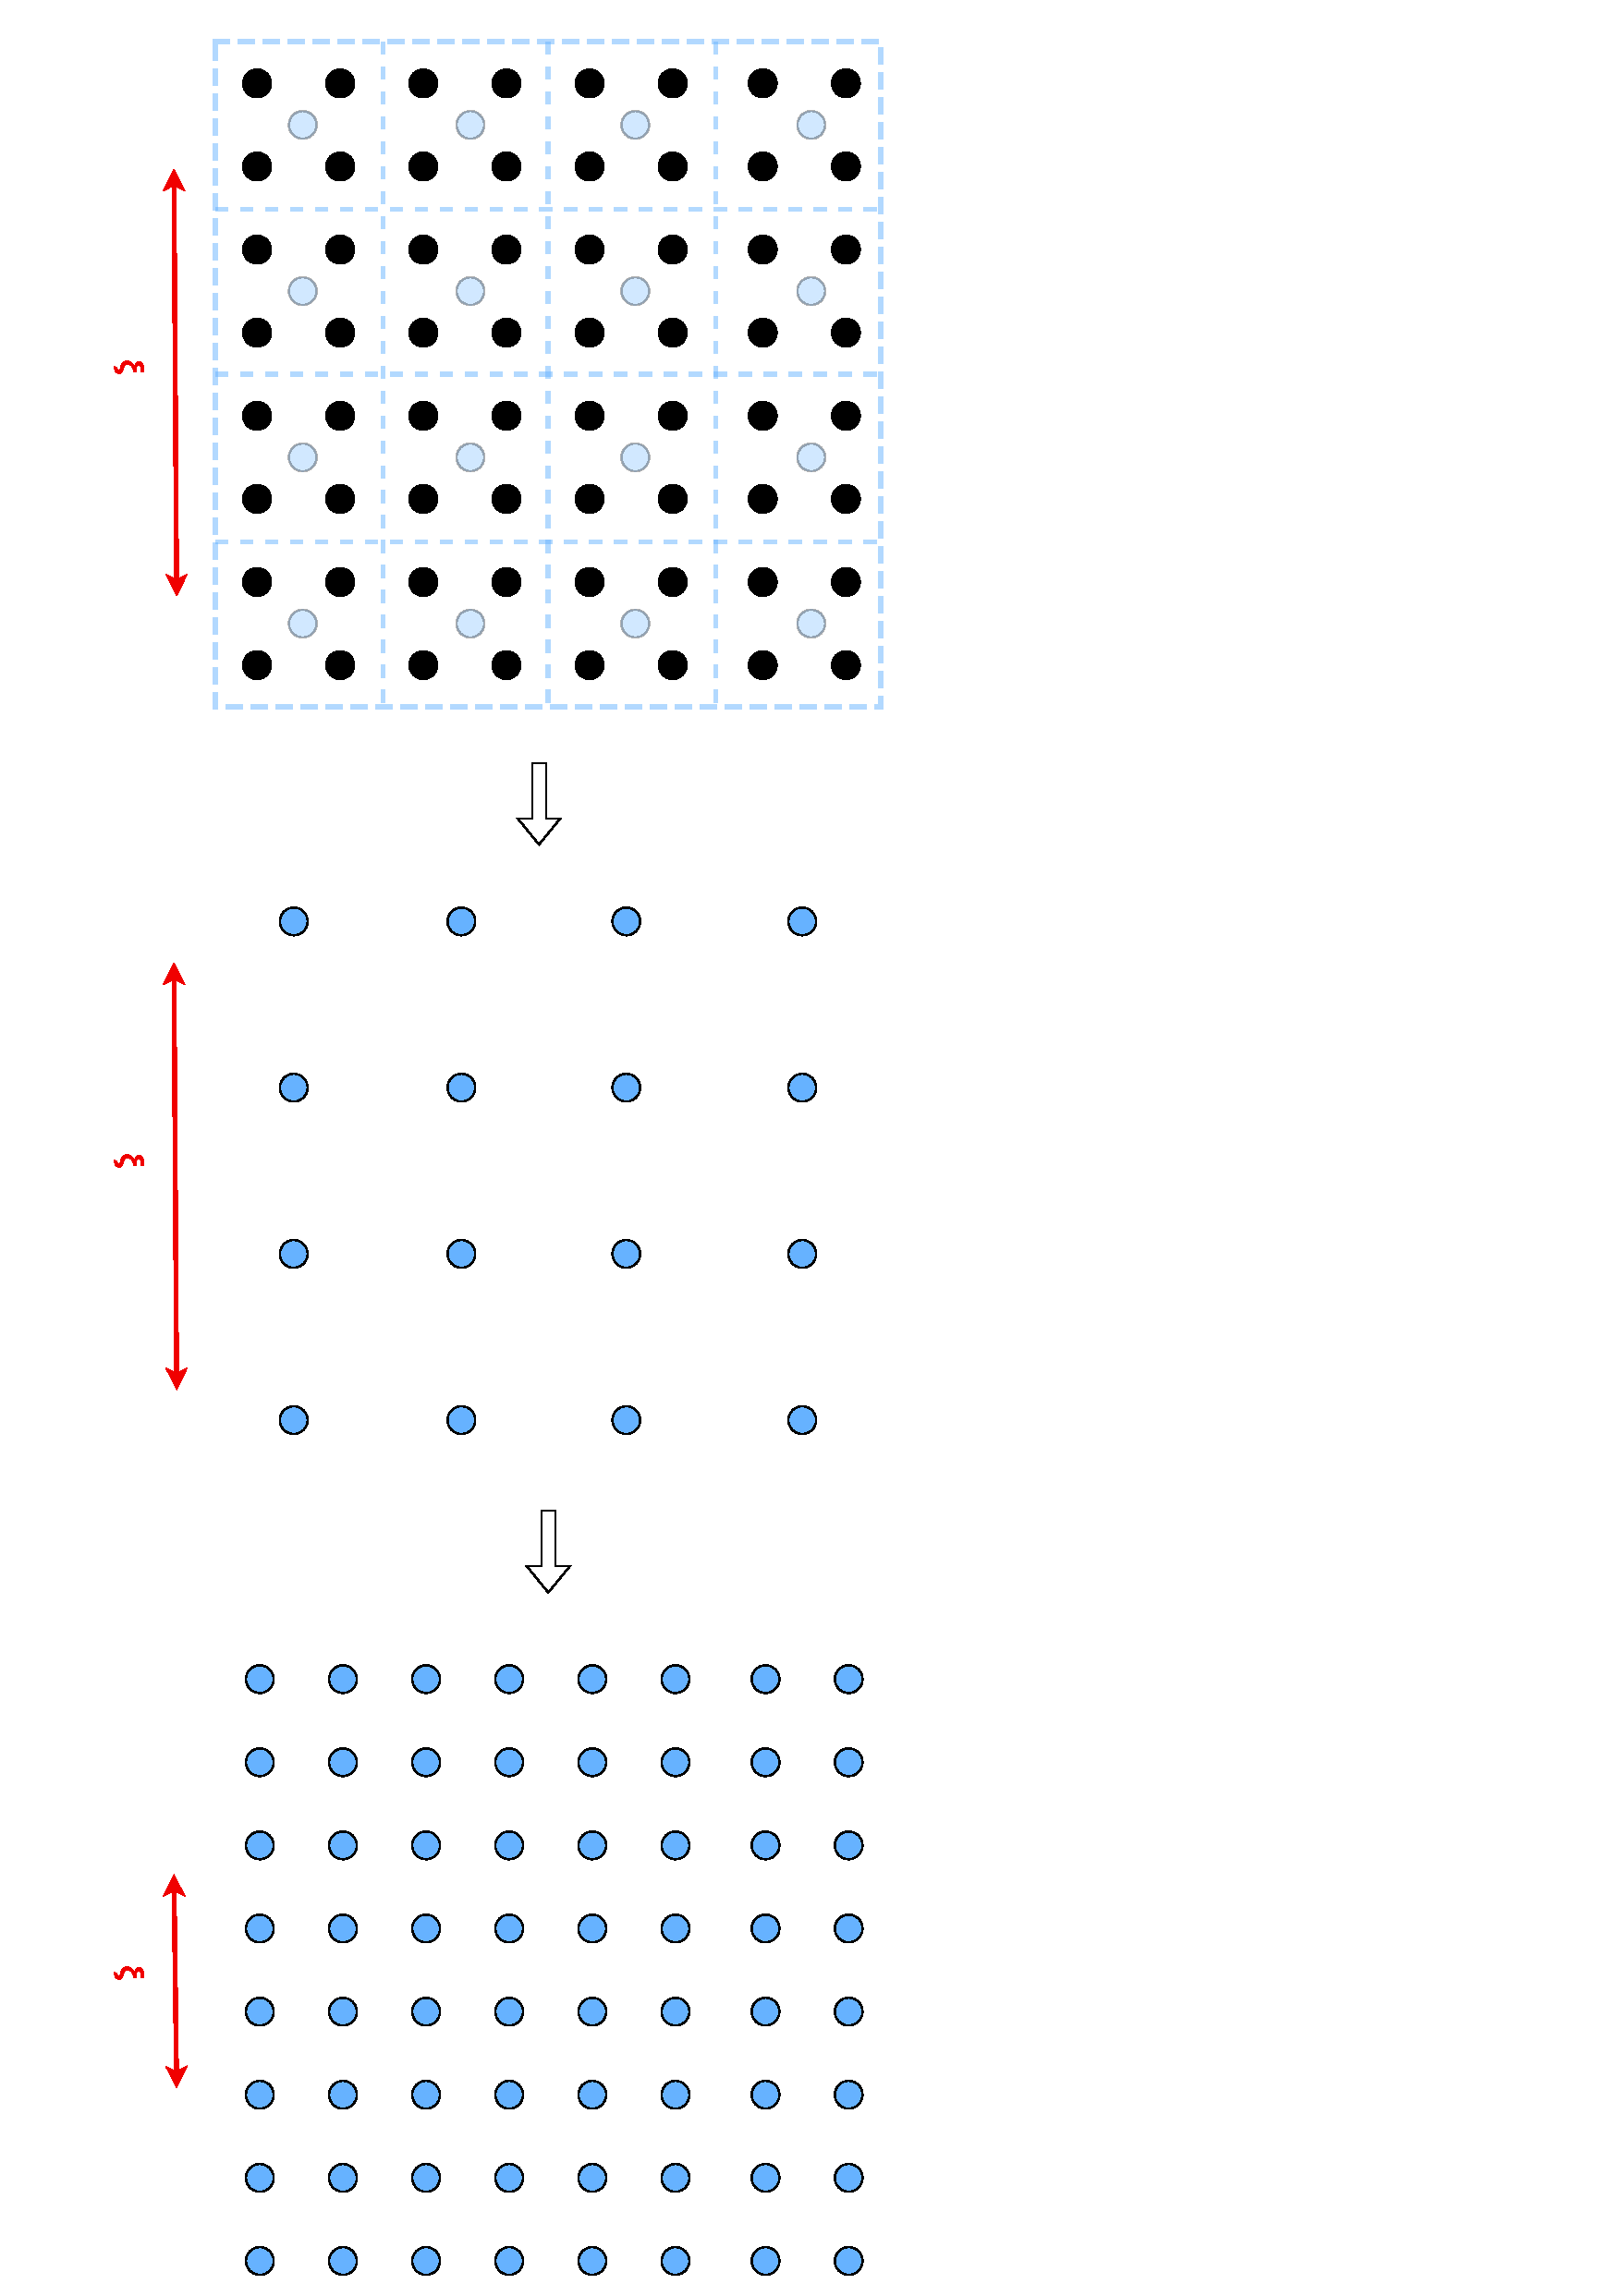
\includegraphics[angle=90,scale=0.34]{figures/blockspin.pdf}
    \caption[Block-spin transformation]{The two steps of the block-spin transformation. The black dots indicate the original field $\phi$, while the blue dots indicate the coarse-grained field $\bar \phi$.}
    \label{fig:blockin_first}
\end{figure}
To illustrate the idea, let us consider a set of spins whose magnetisation is described by a function $\phi(x)$. The spins are located on a discrete lattice $\mathscr{L}$ with spacing $a$, so that the function assumes values only at such sites $\phi(x_i) = \phi_i \neq 0 \Leftrightarrow x_i \in \mathscr{L}$. Suppose then that their interaction is described by a certain action $S[\phi]$ and a partition function
\begin{equation*}
    Z=\sum_{\phi} \mathrm{e}^{-S[\phi]}.
\end{equation*}
We now want to introduce a coarse-grained (or blocked) field $\bar\phi$ within a spacetime cell of volume $\mathcal{V}$. Such a coarse grained field can be defined, for example, as an average over the spins within the cell $\mathcal{V}$. If the spins can only be $0$ or $1$ like in a Ising model, then we might opt for a majority rule \cite{cardy_1996}.
We now want to find a new action $S_b$ such that 
\begin{equation}
    Z=\sum_{\phi} \mathrm{e}^{-S(\phi)}= \sum_{\bar\phi} \mathrm{e}^{-S_b\left(\bar\phi\right)}.
    \label{eq:blocked_action}
\end{equation}
Suppose for the moment that such $S_b$ has been found. The coarse-graining procedure comes with a loss of resolution since the spacing is changed $a \to 2a$. Hence one can rescale distances and momenta in the new action via $a \to a/2, p \to 2p$ and then compare the result with the initial action. This constitutes the second step of the block-spin transformation. \\
The whole procedure can be iterated multiple times, and can be thought as a zoom-out with a corresponding coarse graining, in order to describe the system in terms of the relevant scales as pictured in figure \ref{fig:blockin_first}. As made clear in the picture, the physical correlation length $\xi$ is reduced by the block-spin step, since the description is now in terms of the coarse field $\bar\phi$. 
There are only two exceptions for this, either the correlation length is zero, or infinite. The latter case represents a fixed-point of the RG, and the system exhibits scale invriance. \\
Note that the condition \eqref{eq:blocked_action} is non-trivial. One can, in principle, build an ad-hoc action that fulfills the condition, but it is complicated, since $S_b$ can be also be very different from $S$. For example, if the action $S[\phi]$ contains only nearest-neighbour interactions, the new action $S'[\bar\phi]$ can contain higher order interactions such as nearest-to-nearest neighbour, or even more.  In principle, all the terms compatible with the original symmetries are allowed, and one has often to rely on some approximations. For example, if one is interested in long range properties of the system, and the volume $\mathcal{V}$ is sufficiently small, one can assume 
the functional form of the action $S$ to remain approximately the same, with the the only change due to the dimensional rescaling of dimensionful quantities mentioned above. Thus, as the procedure is iterated and the correlation length scale is approached, one has to take account higher order interactions. For an example of the explicit construction of the RG for an Ising model, see \cite{cardy_1996}.

\subsection{Wilsonian RG}
\label{sec:wilson_rg}
The Wilsonian picture of renormalisation \cite{WilsonRG1,WilsonRG2} is formulated in momentum space and in general is more suitable for theories in the continuum.\\
The idea is that a physical theory observed a energy scale $\Lambda$ can be seen as an effective theory of a more fundamental one, defined at scale $\Lambda_0 > \Lambda$. \\
To see how this can happen, let us consider a theory defined by the action $S[\phi]$ scale $\Lambda_0$, and let us split the field as 
\begin{equation*} 
    \phi = \bar\phi + \varphi
\end{equation*} 
where $\bar\phi$ are fields with momenta $p^2 \leq \Lambda^2$ and $\varphi$ are fields with $\Lambda^2 < p^2 \leq \Lambda_0^{2}$. \\
This allows to split the action as
\begin{equation*} 
    [\bar\phi + \varphi] = S_{\Lambda}[\bar\phi] + \delta S[\bar\phi, \varphi]
\end{equation*}
including all the dependence on $\varphi$ in $\delta S[\bar\phi, \varphi]$. \\
The path integral can be rewritten as
\begin{equation*}
    \begin{aligned}
        Z = \int D\phi \, e^{-S[\phi]} &= \int D\bar\phi_{\Lambda} \, e^{-S_{\Lambda}[\phi]} \int D\varphi  \, e^{-\delta S[\phi, \varphi]}  \\
        &= \int D\bar\phi_{\Lambda} \, e^{-S_{\Lambda}[\bar\phi] - S_\text{UV}[\bar\phi]}\\
        &= \int D\bar\phi_{\Lambda} \, e^{-S_{\Lambda}^\text{eff}[\bar\phi]},
    \end{aligned}
\end{equation*}
where 
\begin{equation*}
    S_{\Lambda}^\text{eff} = S_{\Lambda}[\bar\phi] + S_\text{UV}[\bar\phi], \qquad  S_\text{UV}[\bar\phi] = -\log\left( \int D\varphi \, e^{-S_{\Lambda}[\phi, \varphi]}\right).
\end{equation*}
$ S_\text{UV}[\bar\phi]$ encodes all the information of UV modes with $\Lambda^2 < p^2 \leq \Lambda_0^2$. \\
The action $S_{\Lambda}[\bar\phi]$ has the same functional form of the initial action $S[\phi]$, but it is now defined only for fields with momenta $p^2 \leq \Lambda^{2}$. Instead, $S^\text{eff}_\Lambda[\bar\phi]$ constitutes an effective description of the original theory at scale $\Lambda$ and depends only on degrees of freedom with $p^2 \leq \Lambda^2$. \\
One can then operate a rescaling of distances and momenta to complete the Wilson RG step, according to the parameter 
\begin{equation*}
    s^2 = \Lambda^2 / \Lambda_0^2.
\end{equation*}
If, for example, $d_g$ is the energy dimension of a coupling $g$ in the action, then the rescaling transformation causes 
\begin{equation*} 
    g \to s^{d_g} \, g.
\end{equation*}
The same applies to the fields and other dimensionful quantities. If the corrections from $S_\text{UV}$ are negligible, such as for high cutoff $\Lambda \approx \Lambda_0$, then this is the only contribution to the change in the couplings and fields due to the Wilson step. More in general, for higher order iterations of the procedure, the couplings' dependence on $s$ is caputered by the $\beta$-functions 
\begin{equation*}
    \beta_g = \frac{d}{ds} \, g(s).
\end{equation*}
A full treatment of RG is out of scope here and we ask the reader to consult more appropriate references fore more details \cite{Peskin:1995ev}. \\~\\
At this point, one can clearly see the analogy with the block-spin transformation introduced in the previous section. Performing the integral over high momenta modes
can be thought as performing averages (coarse graining) over neighbours. This causes a loss of resolution which can be recovered by rescaling distances and momenta. The rescaling is essential for a description of fixed points, since it can be pictured as a zoom-out. \\
Therefore, the philosophy of Kadanoff and Wilson approaches was that the blocking transformation reduces the complexity of many-body systems by systematically reducing the number of degrees of freedom being taken into account, without changing the physical content of the
theory \cite{WILSON197475,carosso2020novel}. \\~\\
We want to conclude this section by mentioning that the splitting of the action can be done by writing
\begin{equation*}
    S^\text{eff}_\Lambda[\bar\phi] = S[\phi] + \Delta S_{\Lambda}^{(\mathrm{IR})}[\bar\phi],
\end{equation*}
where $\Delta S_{\Lambda}^{(\mathrm{IR})}[\hat{\phi}]$ is a regulating function which typically assumes the form
\begin{equation} 
    \Delta S_{\Lambda}^{(\mathrm{IR})}[\bar\phi] = \frac{1}{2} \int \frac{\mathrm{d}^d p}{(2 \pi)^d} \bar\phi(-p) \ \Lambda^2 \, \left(\frac{1}{r_{\Lambda}(p^2)}-1\right) \ \bar\phi(p),
\end{equation}
For a sharp momentum cutoff one has
\begin{equation*}
    r_{\Lambda}(p^2) = \theta\left(p^2-\Lambda^2\right).
\end{equation*}
This result will allow for a deep connection between coloured stochastic quantisation and the functional renormalisation group, the latter describing the functional dependence of $S_\Lambda^\text{eff}[\bar\phi]$ on the cutoff scale $\Lambda$ \textcolor{red}{citationsssss}.


\section{Lattice QFT and the continuum limit}
\label{sec:lattice_continuum_}
The starting set up is the euclidean formulation of quantum field theory, where one typically defines a path integral $Z$, which, for a general scalar field $\phi(x)$ and a fermion field $\psi(x)$, assumes the form
\begin{equation}
    Z = \int \mathcal{D}\phi\mathcal{D}\psi\mathcal{D}\bar\psi \ e^{-S[\phi, \psi, \bar\psi]}, \qquad \mathcal{D}\xi = \prod_x d\xi_x, \quad \xi \in \{\phi, \psi, \bar\psi\},
    \label{eq:path_integral_generic}
\end{equation}
and correlation functions are computed via
\begin{equation*}
        \left\langle \xi_{x_1} \dots \xi_{x_n}  \right\rangle = \frac{1}{Z} \int \mathcal{D}\phi\mathcal{D}\psi\mathcal{D}\bar\psi \ \xi_{x_1} \dots \xi_{x_n} \ e^{-S[\phi, \psi, \bar\psi]}, \qquad \xi_{x_i} \in \{\phi_{x_i}, \psi_{x_i}, \bar\psi_{x_i}\}. \\
\end{equation*}
Let us then consider a lattice $\mathscr{L}$, with spacing $a$, and $N_\mu$ points in each spacetime direction $\mu$, hence a physical length $L_\mu = N_\mu \, a$.
For simplicity we restricted here to a scalar field $\phi$ and we will recall fermionic properties only when relevant, but what follows has general validity. 
The action and the path integral measure are now taken over discrete quantities 
\begin{equation*}
    \begin{aligned}
	    S = \int d^dx \, \mathcal{L}(\phi(x)) \qquad &\to \qquad S = a^d \sum_{n \in \mathscr{L}} \, \mathcal{L}(\phi(n)), \\
        \prod_{x} d\phi(x) \qquad &\to  \qquad \prod_{n \in \mathscr{L}} d\phi(n),
    \end{aligned}
\end{equation*}
where $\mathcal{L}(\phi)$ is the Lagrangian density function.  \\
The path integral is hence
\begin{equation*}
    Z = \int \prod_n d\phi(n) \, e^{-S[\phi]},
\end{equation*}
and the probability of a field configuration $\phi$
\begin{equation}
    p(\phi) = \frac{1}{Z} \, e^{-S[\phi]}.
    \label{eq:probability_distribution_lattice}
\end{equation}
Expectation value of observables are computes as
\begin{equation}
    \expect{O(\phi)}  = \frac{1}{Z} \, \int \prod_n d\phi(n) \, O(\phi) \, e^{-S[\phi]}.
    \label{eq:expectation_value_lattice}
\end{equation}
In order to simulate a theory and perform the above sums one has to go to finite volumes and impose boundary conditions. In the space directions, we take periodic conditions 
\begin{equation*}
    \begin{aligned}
        \phi(t, \vec x) &= \phi(t, \vec x + \vec T), \\
        \psi(t, \vec x) &= \psi(t, \vec x + \vec T).
    \end{aligned}
\end{equation*}
Instead, a finite time extent is related to the temperature of the system \cite{le_bellac_1996,rothe_LGT} via
\begin{equation*}
    \beta = 1/T = 1/L_t,
\end{equation*}
and boundary conditions are chosen depending on the spin-statistic of the corresponding particles, namely periodic conditions for bosons, and anti-periodic for fermions
\begin{equation*}
    \begin{aligned}
        \phi(t, \vec x) &= \phi(t + T, \vec x) \qquad \text{bosons}, \\
        \psi(t, \vec x) &= -\psi(t + T, \vec x) \quad \text{fermions}.
    \end{aligned}
\end{equation*}
Such a formulation naturally brings a momentum cutoff $\Lambda = \pi/a$ since now all the momenta are restricted to the first Brilloune zone $p_\mu \in [-\pi/a, \pi/a]$. \\~\\
To compute observables one relies on Monte-Carlo methods to generate field configurations, sampling the distribution \eqref{eq:probability_distribution_lattice} and convergence to the statistical value given by \eqref{eq:expectation_value_lattice} is expected in the limit of infinite samples $N_\text{samp} \to \infty$. \\
To recover the continuum results, one has to take $V \to \infty, a \to 0$ \footnote{the order here is important, see for example \cite{seiler,friedli_velenik_2017}}, but this task cannot be done so straightforwardly.
Continuum limits of lattice theories are intimately connected to the existence of critical points. To see why this is the case, consider the dimensionless mass gap 
\begin{equation*}   
    \hat\xi = m \, a
\end{equation*} 
of a certain theory. The quantity $\xi$ is also called correlation length and it is related to the exponential decay of correlation functions between local observables measured
at different points on the lattice, as given by \textcolor{red}{add ref. eq.}\\
When taking the continuum limit we want $a \to 0$, while having a finite physical mass $m$. This implies that the correlation length $\hat \xi$ has to diverge: in the language of statistical physics, this is a second order phase transition. Of course to bring the system at its critical point, where such phase transition happens, one has to tune the bare parameters $g_0^i$ of the theory to their critical values $g_0^{i \, *}$. 
To do this, one should find the zeros of the lattice beta functions
\begin{equation*}
    \beta_g^\text{latt} = a \frac{d}{da} g(a) \overset{!}{=} 0, \qquad a = \pi/\Lambda.
\end{equation*}
As this is quite hard task to do on the lattice, one typically relies on some approximation schemes such as employing perturbative continuum beta functions. \\
In any case, from this description it should be clear that the spacing $a$ should not be treated as a free parameter in the continuum limit, but rather a dynamically determined quantity that depends on the couplings of the theory.\\~\\
Note that in the limit $a \to 0$, one has $\Lambda \to \infty$. If one's scope is to simulate an effective theory which is expected to hold only up to a scale $\Lambda_\text{phys}$, one must have $\Lambda \leq \Lambda_\text{phys}$, with a consequent lower bound on the lattice spacing $a \geq a_\text{phys} = \pi / \Lambda_\text{phys}$. \\ ~

\section{Stochastic quantisation}
\label{sec:stochastic_quantisation}
The idea of stochastic quantisation \cite{ParisiWu,Damgaard1987StochasticQuantization} is that Euclidean Quantum Field theory can be thought as a system in thermal equilibrium with a heat reservoir and hence described as a stochastic process via the Langevin equation. For this, one has to introduce a fictitious time variable $\tau$ that labels the state $\phi(\tau, x)$ of the system 
during the evolution. \\
\subsection{Standard stochastic quantisation}
Let us consider, for example, a scalar field $\phi$ with a Euclidean action $S[\phi]$ and the following Langevin equation
\begin{equation}
    \partial_\tau \phi(\tau, x) = - \frac{\delta S[\phi]}{\delta \phi (\tau, x)} + \eta (\tau, x),
    \label{eq:Langevin_scalar_full}
\end{equation}
where $K_{\phi}(\tau) \equiv -\delta S[\phi]/\delta \phi (\tau, x)$ is the drift term and $\eta (\tau, x)$ is a random white noise field assumed to be normally distributed
\begin{equation*}
    P(\eta) = \frac{\exp\left(-\frac{1}{4}\int_{\tau,x} \eta^2(\tau, x)\right)}{\int D\eta \exp\left(-\frac{1}{4}\int_{\tau,x} \eta^2(\tau,x)\right)},
\end{equation*} 
which, in particular, implies
\begin{equation}
    \expect{\eta(x,\tau)} = 0, \qquad \expect{\eta(x,\tau) \, \eta(x',\tau')} = 2 \, \delta(x - x') \, \delta (\tau - \tau').
    \label{eq:white_noise_definition}
\end{equation}
Stochastic average with respect to the measure $P(\eta)$ are computed via 
\begin{equation*}
    \expect{A(\eta)} = \int D\eta \, P(\eta) \, A(\eta).
\end{equation*}
In momentum space, \eqref{eq:white_noise_definition} becomes
\begin{equation}
    \begin{aligned}
        \expect{\eta(p,\tau)} &= \expect{\int_x e^{ipx}\eta(x,\tau)} = \int_x \expect{e^{ipx}\eta(x,\tau)} = 0, \\
        \expect{\eta(p,\tau)\eta(q,\tau')} &= \expect{\int_{xy} e^{ipx + iqy} \eta(x,\tau)\eta(y,\tau')} \\
        &= \int_{xy} e^{ipx + iqy} \expect{\eta(x,\tau)\eta(y,\tau')} \\
        &= 2 \, (2\pi)^2 \, \delta(p + q) \, \delta(\tau - \tau').
    \end{aligned}
    \label{eq:white_noise_definition_momentum}
\end{equation}
In absence of the noise term $\eta(\tau,x)$, equation \eqref{eq:Langevin_scalar_full} simply represents an evolution of the field towards the minimum of the action, and at equilibrium the field is constrained to $\partial_\tau \phi(x,\tau) = 0 = \delta S[\phi]/\delta \phi (\tau, x)$, namely to the classical equations of motion.\\
For any observable $O$, which is function of the field, one has, for fixed time $\tau$,
\begin{equation*}
    \expect{O(\phi(\tau))} = \int D\eta \, P(\eta) \, O(\phi(\tau)),
\end{equation*}
from which it follows straightforwardly using the Langevin equation and $\expect{\eta} = 0$
\begin{equation*}
    \frac{d}{d\tau} \expect{O(\phi(\tau))} = \expect{\frac{\delta O}{\delta \phi(\tau, x)} \ \partial_\tau \phi(\tau, x)} = -\expect{\frac{\delta O}{\delta \phi}(\tau, x) \ \frac{\delta S}{\delta \phi(\tau, x)}}.
\end{equation*}
It follows trivially that for $O(\phi(\tau)) = \phi(\tau, x)$
\begin{equation*}
        \frac{d}{d\tau} \expect{\phi(\tau, x)} = -\expect{\frac{\delta S}{\delta \phi(\tau, x)}} \quad \underset{Equilibrium}{\Longrightarrow} \quad \expect{\frac{\delta S}{\delta \phi(\tau, x)}} = 0.
\end{equation*}
This also provides a consistency check for the correct implementation of the simulation, since the drift $K_\phi = -\delta S / \delta \phi$ is computed numerically during the evolution. \\
More generally, one can derive a correspondent Fokker-Planck equation \cite{gardiner}, which can be proven to have a stationary distribution if the action is bounded from below, given by \cite{Damgaard1987StochasticQuantization}
\begin{equation}
    \mathcal{P}(\phi) = \frac{1}{Z} \, \exp\left(-S[\phi]\right).
    \label{eq:probability_field_configuration_full}
\end{equation}
This allows one to compute correlation functions as moments of the  probability distribution \eqref{eq:probability_field_configuration_full}. In particular, one has 
\begin{equation}
    \expect{O}_{P(\eta)} = \expect{O}_{\mathcal{P}(\phi)} \equiv \expect{O}.
    \label{eq:expectation_observables}
\end{equation}

\subsection{Stochastic quantisation with coloured noise}
\label{sec:coloured_noise}
In the stochastic quantisation procedure the noise which accounts for the quantum fluctuations of the theory is assumed to be white, as defined in equations \eqref{eq:white_noise_definition}, \eqref{eq:white_noise_definition_momentum}. 
We now want to examine the dynamics in presence of a coloured noise, writing the Langevin equation as
\begin{equation*}
    \partial_\tau \phi(x, \tau) = - \frac{\delta S[\phi]}{\delta \phi (\tau, x)} + \eta_\text{col}(x, \tau),
    \label{eq:Langevin_scalar_regularised}
\end{equation*}
with $\eta_\text{col}(x,\tau) = r_\Lambda(x) \, \eta(x,\tau)$. In particular, here we restrict to the regulating function defined as a sharp cutoff in momentum space
\begin{equation}
    r_\Lambda(p) = \theta(\Lambda^2 - p^2),
    \label{eq:regulator}
\end{equation}
and we invite the reader to consult \cite{Pawlowski2017CoolingNoise} for a discussion of other regulating functions. \\
The noise field in momentum space is then
\begin{equation*}
    \begin{aligned}
        \eta_\text{col}(p, \tau) &= \mathcal{F}[\eta_\text{col}(x,\tau)] = \mathcal{F}[r_\Lambda(x,\tau) \eta(x,\tau)] = \mathcal{F}[r_\Lambda(x,\tau)] \star \mathcal{F}[\eta(x,\tau)] \\
        &= \theta(\Lambda^2 - p^2)  \, \eta(p, \tau).
    \end{aligned}
\end{equation*}
where $\mathcal{F}$ indicates the Fourier transform and $\star$ the convolution product. \\
An interesting quantity to look at is the position-space noise correlation function
\begin{equation}
    \begin{aligned}
        C_{\eta}(x,\tau,y,\tau') &= \left\langle\eta_\text{col}(x,\tau) \, \eta_\text{col}(y,\tau')\right\rangle \\
        &= \frac{1}{(2\pi)^{4}} \int D\eta \, P(\eta) \left[\int_{p,q} e^{-ipx-iqy }\eta_\text{col}(p,\tau) \, \eta_\text{col}(q,\tau')\right] \\
        &= \frac{1}{(2\pi)^{4}} \int_{p,q} e^{-ipx-iqy } \int D\eta \left[ P(\eta) \, \eta(p,\tau) \, \eta(q,\tau') \right] \\
        &\qquad\times \theta(\Lambda^2 - p^2) \, \theta(\Lambda^2 - q^2)  \\
        &= \frac{2}{(2\pi)^{2}} \int_{p,q} e^{-ipx-iqy} \, \delta(p+q) \, \theta(\Lambda^2 - p^2) \, \theta(\Lambda^2 - q^2) \, \delta(\tau - \tau') \\
        &= \frac{2}{(2\pi)^{2}} \int_{p} e^{-ip(x-y)} \, \theta(\Lambda^2 - p^2) = \frac{1}{\pi} \, \int_0^\Lambda \, d\omega \, \omega \, J_0(\omega |x-y|),
    \end{aligned}
    \label{eq:coloured_noise_correlation}
\end{equation}
where $J_0(x)$ is a Bessel function of the first order. The integral in the last line is computed numerically as a function of $d=|x-y|$ and reported in figure \ref{fig:bessel} for three different values of the cutoff $\Lambda_1 < \Lambda_2 < \Lambda_3$. This shows nicely that for $|x-y| \ll 1/\Lambda$ the noise is now correlated, while for $|x-y| \gg 1/\Lambda$ the correlation function vanishes, as in the white noise case. In other words, only the short-length behaviour of the system is affected by the introduction of such a regulating term, as one could expect.\\~\\
\begin{figure}
    \centering
    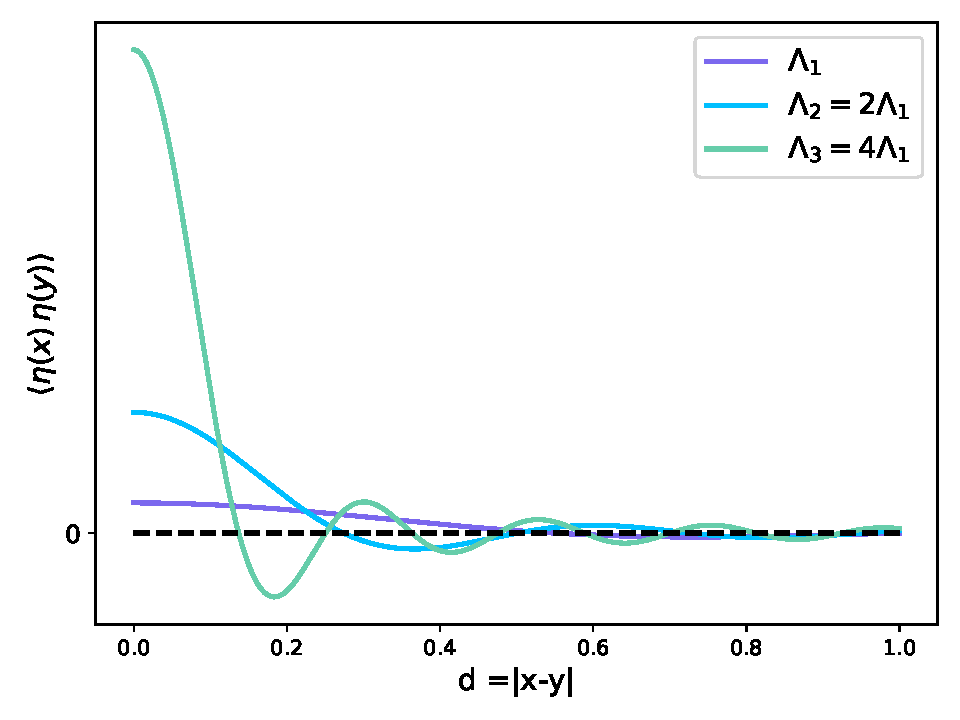
\includegraphics[scale=0.6]{figures/bessel.pdf}
    \caption[Correlated noise]{Noise correlation as a function of $d=|x-y|$ for three different values of the cutoff $\Lambda_1 < \Lambda_2 < \Lambda_3$, in arbitrary units. The plot is qualitative, but shows clearly that with a regulated noise, only the short-distance behaviour is affected.}
    \label{fig:bessel}
\end{figure}
Another intuitive and interesting aspect of the dynamics in the presence of coloured noise can be deduce by looking at the field expression in terms of the retarded Langevin Green function \cite{Damgaard1987StochasticQuantization}, which is here not derived, but reported from \cite{Pawlowski2017CoolingNoise}
\begin{equation*}
        \phi(x, \tau) = \int_{x^{\prime}} \int_{-\infty}^\tau \mathrm{d} \tau^{\prime} G\left(x-x^{\prime}, \tau-\tau^{\prime}\right) \, \left[r_{\Lambda}\left(\Delta_x\right) \eta\left(x, \tau^{\prime}\right)-\frac{\delta S}{\delta \phi}|_{p=0} \, \phi\left(x^{\prime}, \tau\right)\right],
\end{equation*}
where
\begin{equation*}
    G\left(x-x^{\prime}, \tau-\tau^{\prime}\right) =\theta\left(\tau-\tau^{\prime}\right) \int_p \mathrm{e}^{-i p \cdot\left(x-x^{\prime}\right)} \mathrm{e}^{-\left(\tau-\tau^{\prime}\right)\left(p^2+m^2\right)}.
\end{equation*}
By looking at the first term in the square bracket, one can conclude that there is no propagation of modes with momentum $p^2\geq \Lambda^2$ due to the noise term, but one can still have contribution from modes $p^2 > \Lambda^2$ from the second term, which corresponds to the deterministic part of the equations of motion. Stated differently, UV quantum fluctuations with $p^2 > \Lambda^2$ are removed from the dynamics of $\phi$, but still contribute classically. \\~\\
Generally speaking, the stationary distribution probability of the regulated stochastic process is given by \cite{Pawlowski2017CoolingNoise}
\begin{equation}
    \mathcal{P}_\Lambda(\phi) = \frac{1}{Z} \, \exp\left(-S_\Lambda[\phi]\right) = \frac{1}{Z} \, \exp\left(-(S[\phi] + \Delta S_\Lambda[\phi])\right),
    \label{eq:probability_field_configuration_regularised}
\end{equation}
where the correction term $\Delta S_\Lambda[\phi]$, reads, for a regulator $r_\Lambda(p^2)$,
\begin{equation*}
        \Delta S_{\Lambda}[\phi]=\frac{1}{2} \int_p \phi_p \, \Lambda^2\left(\frac{1}{r_{\Lambda}\left(p^2\right)}-1\right) \, \phi_{-p}.
\end{equation*}
\textcolor{red}{at this point mention that this is the stationary pdf that one gets with frg for sharp cutoff, and cite some papers.}

\section{Chiral symmetry}
\label{sec:chiral_symmetry}
In this section we want to introduce chiral symmetry and its breaking, both in the continuum and on the lattice. \\
It is useful to adopt the notation 
\begin{equation*}
    \psi = (\psi^{(1)}, \dots, \psi^{(N_f)}).
\end{equation*} 
We then introduce left-handed and right-handed spinors
\begin{equation*}
	\psi_L = (1-\gamma_5) \, \psi, \qquad \psi_R = (1+\gamma_5) \, \psi,
\end{equation*}
for which
\begin{equation*}
	\psi = \frac{(1-\gamma_5)}{2} \psi + \frac{(1+\gamma_5)}{2} \psi = \psi_L + \psi_R.
\end{equation*}


\subsection{Chiral symmetry in the continuum}

The free massless Dirac Lagrangian
\begin{equation} 
    \mathcal{L}_D = \bar\psi \slashed{\partial} \psi = \bar\psi_L \slashed{\partial} \psi_L + \bar\psi_R \slashed{\partial} \psi_R
\end{equation} 
is symmetric under the chiral group $SU(N_f) _L\times SU(N_f)_R$, namely
\begin{equation*}
	\begin{aligned}
		\psi_L(x) \to U_L\psi_L(x), &\qquad \bar\psi_L(x) \to \bar\psi_L(x) U_L^{\dagger}, \\
		\psi_R(x) \to U_R\psi_R(x), &\qquad \bar\psi_R(x) \to \bar\psi_R(x) U_R^{\dagger},
	\end{aligned}
\end{equation*}
for $U_L, U_R \in SU(N_f)$. \\
In terms of the full spinor $\psi$, the chiral symmetry can be written as 
\begin{equation*} 
    \psi \to M \, \psi, \qquad \bar\psi \to \bar\psi,
\end{equation*} 
where
\begin{equation*}
    M = e^{i(\theta_a \tau^a + \gamma_5 \beta_a\tau^a)}, \quad \tau^a \in su(N_f)
\end{equation*}
so that 
\begin{equation*} 
    SU(N_f) _L\times SU(N_f)_R \simeq SU(N_f)_V \times SU(N_f)_A.
\end{equation*}
$SU(N_f)_V$ is the isospin subgroup, characterised by $\beta_a =0$, and $SU(N_f)_A$ is the axial rotation subgroup, characterised by $\theta_a = 0$. \\
To be more precise, the full invariance group of the classical action is
\begin{equation*}
    SU(N_f)_L \times SU(N_f)_R \times U(1)_A \times U(1)_V,
\end{equation*}
where the axial and vector symmetry transformations are, respectively,
\begin{equation*}
        \psi \to e^{i\theta \gamma_5} \, \psi, \qquad \psi \to e^{i\theta} \, \psi.
\end{equation*} 
One can thus prove that axial symmetry is broken by quantum anomalies (see for example \cite{schwartz}), so that the symmetry in the quantum case is
\begin{equation*}
    SU(N_f)_L \times SU(N_f)_R \times U(1)_V.
\end{equation*}
If equal masses for each flavour are introduced, then the symmetry group reduces to the isospin subgroup, diagonal in flavour space
\begin{equation*}
    SU(N_f)_V \times U(1)_V.
\end{equation*}
Finally, if the fermions have different masses, the symmetry group reduces to 
\begin{equation*}
    \underbrace{U(1) \times \dots \times U(1)}_{N_f} \times U(1)_V.
\end{equation*}

\subsection{Chiral symmetry on the lattice}
The essence of chiral symmetry for fermions can be expressed as \cite{gattringer_LQCD}
\begin{equation}
    \left\{\gamma_5, D \right\} = 0
    \label{eq:chiral_symmetry}
\end{equation}
Implementing chiral symmetry on a finite-volume spacetime lattice, is a hard task. This is because, as proven by Nielsen and Ninomiya \cite{NIELSEN198120}, one either has chiral symmetry on the lattice, or solves the doubling problem. \\
In particular, the insertion of the Wilson term in the action, as shown in Appendix \ref{chap:AppendixB}, causes explicit breaking of the chiral symmetry. If one's goal is to study spontaneous symmetry breaking, this constitues a problem. 
Thus, many options have been proposed to circumvent the issue. As an example we mention the approach by Ginsparg and Wilson \textcolor{red}{citationsssss}, who proposed to modify the chiral symmetry condition \eqref{sec:chiral_symmetry} to 
\begin{equation*}
    \left\{\gamma_5, D \right\} = a \, D \gamma_5 D
\end{equation*}
The right hand-side of the equation vanishes in the continuum limit $a \to 0$. In this way, one can define chiral symmetry on the lattice remaining consistent in the continuum limit. This approach will not be pursued further and we ask the reader to consult 
appropriate references \cite{rothe_LGT,gattringer_LQCD} for a detailed treatment. \\
Our approach to study chiral symmetry will be discussed and motivated in section \ref{sec:chiral_PT}.

\section{Yukawa theory}
\label{sec:Yukawa_theory}

\subsection{Description of the model}
Let us consider the Yukawa theory defined by the action
\begin{equation}
\begin{aligned}
    S[\phi,\psi,\bar\psi] &= S_\phi[\phi] + S_\psi[\psi, \bar\psi] + S_\text{int}[\phi, \psi, \bar\psi], \\
     S_\phi[\phi] &= \int_x \phi_x \left(-\frac{\partial^2_x}{2} + \frac{m_\phi^2}{2}\right) \phi_x + \frac{\lambda}{4!} \, \phi_x^4, \\
     S_\psi[\psi, \bar\psi] &= \int_x \sum_{f=1}^{N_f} \bar \psi_x^{(f)} \left(\slashed{\partial}_x + m_q \right) \psi_x^{(f)}, \\
     S_\text{int}[\phi, \psi, \bar\psi] &= \int_x \sum_{f=1}^{N_f} g \, \bar \psi_x^{(f)} \, \phi_x \, \psi_x^{(f)}.
    \label{eq:full_action_continuum}
\end{aligned}
\end{equation}
One can see that the action is made of a scalar part $S_\phi[\phi]$, a fermionic part $S_\psi[\psi, \bar\psi]$ and a Yukawa interaction term $S_\text{int}[\phi, \psi, \bar\psi]$. \\
In pratice we will work with fixed number of flavours $N_f = 2$, but it is useful to keep track of $N_f$ and set it to its value when needed. \\
It is also convenient for later purposes to define the operators $K, D$ represented in position space as 
\begin{equation}
    \begin{aligned}
        K(x, y) &=  \left(-\partial^2_x + m_\phi^2\right) \ \delta(x,y), \\
        D(x, y) &= \left(\slashed{\partial}_x + m_q + g\phi \right) \ \delta(x,y),
    \end{aligned}
    \label{eq:definition_kinetic_terms_continuum_position}
\end{equation}
and in momentum space as
\begin{equation}
    \begin{aligned}
        \widetilde{K}(p, q) &=  \int_{x,y} e^{-ipx} \left(\partial^2_x + m_\phi^2\right) \ \delta(x,y) \ e^{iqy} = \left(\frac{p^2}{2} + \frac{m_\phi^2}{2}\right) \ \delta(p,q), \\
        \widetilde{D}(p, q) &= \int_{x,y} e^{-ipx} \left(\slashed{\partial}_x + m_q + g\phi \right) \ \delta(x,y) \ e^{iqy} = \left(\slashed{p}_x + m_q + g\phi \right) \ \delta(p,q).
    \end{aligned}
    \label{eq:definition_kinetic_terms_continuum_momentum}
\end{equation}
This allows one to rewrite the action as
\begin{equation*}
    S[\phi,\psi,\bar\psi] = \int_x \frac{1}{2} \, \phi_x \, K_{xx} \, \phi_x + \frac{\lambda}{4!} \, \phi_x^4 + \sum_{f=1}^{N_f} \bar\psi_x^{(f)} \, D_{xx} \, \psi_x^{(f)}.
\end{equation*}

\subsection{Chiral symmetry in the Yukawa model}
The action written in terms of $\psi_L, \psi_R$, reads
\begin{equation}
	S = S_\phi +  \int_x \left[\bar\psi_L \, D \, \psi_L + \bar\psi_R \, D \, \psi_R + (m_q + g\phi) \,  \left(\bar\psi_L\psi_R + \bar\psi_R\psi_L\right)\right].
	\label{eq:action_chirality_explicit}
\end{equation}
The action is not invariant under the full chiral group, but if $m_q = 0$ it is symmetric under the discrete chiral transformation
\begin{equation*}
    \begin{aligned}
        \phi &\to -\phi, \\
        \psi_L \to \gamma_5 \psi_L, &\qquad \bar\psi_L \to -\bar\psi_L\gamma_5, \\
        \psi_R \to \gamma_5 \psi_R, &\qquad \bar\psi_R \to -\bar\psi_R\gamma_5,
    \end{aligned}
\end{equation*}
which was first introduced in the Gross-Neveu model \textcolor{red}{citationsssss}. In order to generalise the model to the full chiral group, one has to consider an $O(4)$ scalar sector and interactions, since $O(4) \simeq SU(2) \times SU(2)$. Similar effective theories with such properties are, for example, 
the Nambu-Jona-Lasinio model and the Quark-Meson model \textcolor{red}{citationssssss}. Thus, since we are in $1+1$ dimensions, spontaneous breaking of continuous symmetries is forbidden by the Mermin-Wagner theorem \textcolor{red}{citationsssss}, and we decided to opt for a simple Yukawa theory. \\~\\
We now want to discuss more in detail the phenomenom of (discrete) chiral symmetry breaking and how it can happen in the model. In fact, the latter can happen either
explicitly in the classical action, if a finite quark mass is added, or spontaneously, if $\expect{\phi} \neq 0$. \\
To better see this, let us perform the fermionic path integral explicitly
\begin{equation*}
    \int \mathcal{D} \bar\psi \mathcal{D} \psi \ \exp\left( - \int_x \sum_{f=1}^{N_f} \bar\psi_x^{(f)} \,  D \, \psi_x^{(f)} \right) = (\text{det} \, D[\phi])^{N_f} = e^{N_f\tr \log (D[\phi])},
\end{equation*}
where the trace is performed over spacetime and spinor components. \\ 
The full path integral can now be expressed in terms of the resulting effective action for the scalar fields
\begin{equation*}
    Z = \int \mathcal{D}\phi \ e^{-S_\text{eff}[\phi]},
\end{equation*}
with
\begin{equation}
    S_\text{eff}[\phi] = S_{\phi}[\phi] - N_f \, \underset{x,s}{\tr} \log D[\phi].
    \label{eq:effective_action_no_fermions}
\end{equation}
One can derive the classical equations of motion by imposing $\frac{\delta S}{\delta \phi} = 0$, here expressed in momentum space
\begin{equation}
     (k^2 + m_\phi^2) \, \phi(x) + \frac{\lambda}{6} \, \phi^3(x) = N_f \, g \ \underset{s}{\tr} \left[D^{-1}(\phi(x))\right] = - N_f \, g \ \bar\psi(x) \psi(x)
     \label{eq:classical_EOM_full}
\end{equation}
For $\lambda = 0$, they highlight a simple proportionality relation between magnetisation and chiral condensate, which reads
\begin{equation}
    \phi = - \frac{N_f \, g}{k^2 + m_\phi^2} \ \bar \psi\psi.
    \label{eq:classical_EOM}
\end{equation}
This relation, which was here derived at the classical level, is proven to hold also in mean field on the quantum level \cite{Ayala2021QCDDescriptions} and makes apparent the role of $\phi$ as a quark bilinear. \\
When bosons self-interactions are added, namely when $\lambda \neq 0$, the full relation between $\phi$ and the chiral condensate $\bar\psi\psi$ is given by \eqref{eq:classical_EOM}, but still one expects, qualitatively,
\begin{equation}
    \expect{\phi} \sim \expect{\bar\psi\psi}.
    \label{eq:qualitative_relation_condensate_magnetisation}
\end{equation}
A non-vanishing condensate is also related to a physical quark mass \cite{Ayala2021QCDDescriptions,MANOHAR1984189}, while the presence of magnetisation causes the breaking of $O(1)$ symmetry.
If $\expect{\phi} = v$, one can write $\phi(x) = v + \varphi(x)$ and the massless lagrangian assumes the form 
\begin{equation}
	S = S_\phi +  \int_x \left[\bar\psi_L \, D \, \psi_L + \bar\psi_R \, D \, \psi_R + gv \, \left(\bar\psi_L\psi_R + \bar\psi_R\psi_L\right)\right] + g\varphi(x) \, \left(\bar\psi_L\psi_R + \bar\psi_R\psi_L\right)
	\label{eq:background_field}
\end{equation}
hence showing that one can expect
\begin{equation}
    \expect{\phi} \sim \expect{\bar\psi\psi} \sim m_q.
    \label{eq:qualitative_relation_condensate_magnetisation_mass}
\end{equation}

\begin{figure}
\centering
\begin{minipage}{0.45\textwidth}
    \begin{tikzpicture}[scale=0.8]
        \begin{axis} [axis lines=center, xtick=\empty, ytick=\empty, xlabel=$\phi$, ylabel=$V(\phi)$,
        every axis x label/.style={
            at={(ticklabel* cs:1.0)},
            anchor=west,
        },
        every axis y label/.style={
            at={(ticklabel* cs:1.0)},
            anchor=south,
        },]
            \addplot [domain=-3:3, smooth, thick, color=blue] { 6*x^2 + x^4 - 10*x };
            \addplot [domain=-3:3, smooth, thick, color=green] { 6*x^2 + x^4};
        \end{axis}
     
    \end{tikzpicture}
\end{minipage}
\hfill
\begin{minipage}{0.45\textwidth}
    \begin{tikzpicture}[scale=0.8]
        \begin{axis} [axis lines=center, xtick=\empty, ytick=\empty, xlabel=$\phi$, ylabel=$V(\phi)$,
        every axis x label/.style={
            at={(ticklabel* cs:1.0)},
            anchor=west,
        },
        every axis y label/.style={
            at={(ticklabel* cs:1.0)},
            anchor=south,
        },]
            \addplot [domain=-3:3, smooth, thick, color=blue] { -6*x^2 + x^4 - 5*x };
            \addplot [domain=-3:3, smooth, thick, color=green] { -6*x^2 + x^4};
        \end{axis}
     
    \end{tikzpicture}
\end{minipage}
\label{fig:breaking_O1_symmetry}
\caption[Classical potential and symmetry breaking]{The introduction of the boson-fermion interaction, with a finite fermionic mass, causes explicit breaking of chiral symmetry, with consequence spontaneous breaking of the O(1) symmetry according to \eqref{eq:qualitative_relation_condensate_magnetisation}. It shifts the equilibrium position in the symmetric phase (left) causing $\left\langle \phi \right\rangle \neq 0$, and tilts the potential in the broken phase (right), making the two minima not equivalent.}
\end{figure}

\subsection{Phase structure and order parameters}
\begin{figure}
    \centering
    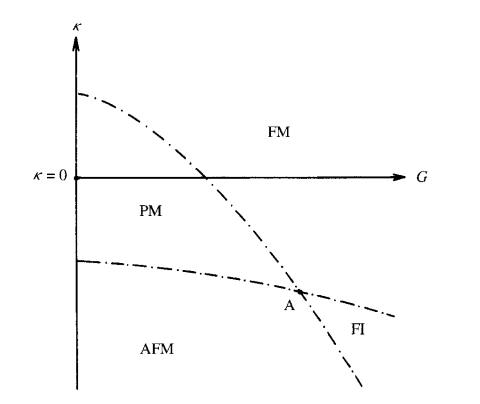
\includegraphics[scale=0.5]{figures/yukawa_phase_diagram.png}
    \caption[Yukawa phase diagram]{General phase diagram of a Yukawa theory. \\ \textcolor{blue}{I know that I wouldn't be allowed to use this picture, I will see later what to do.}}
    \label{fig:yukawa_phase_diagram}
\end{figure}
We want to conclude this chapter by commenting on the phase strcture of the Yukawa theory. This will guide the choice of parameters for the investigation carried in the remaining sections. A sketch of the different phases of the model is reported in figure \ref{fig:yukawa_phase_diagram}. 
The order parameters are the magnetisation $M = \expect{\phi}$ and the staggered magnetisation $M_s = \expect{\Phi}$, where
\begin{equation}
    {\Phi}_x \equiv(-1)^{t+x} \phi_x=\mathrm{e}^{\mathrm{i} \pi\left(t+x\right)} \phi_x .
\end{equation}
The four different phases are characterised by the following combinations of the order parameters
\begin{itemize}
    \item paramagnetic phase: $M = 0, M_s = 0$,
    \item ferromagnetic phase: $M \neq 0, M_s = 0$,
    \item anti-ferromagnetic phase: $M = 0, M_s \neq 0$,
    \item ferrimagnetic phase: $M \neq 0, M_s \neq 0$.
\end{itemize}
The lattice observables used for the investigation are introduced in section \ref{sec:observables}.

% !TeX root = ../main.tex

\chapter{Methods and algorithms}
\label{chapt:methods}

\section{Discretisation of the Yukawa theory}
\label{sec:lattice_discretisation}
In order to make the theory suitable for a numerical simulation on a computer, the continuum formulation of the Yukawa model, which has been introduced in section \ref{sec:Yukawa_theory}, has to be discretised. Here we provided a sketch of a discretisation procedure, and we refer to other resources \cite{CITATIONS} for further details. \\~\\
For what concerns the bosonic part of the action, a discretisation can be done straightforwardly with the following replacements
\begin{equation*}
    \begin{aligned}
        \int_x \quad &\to \quad a^2 \sum_x \\
        \partial^2_x = \frac{\partial^2}{\partial t^2} + \frac{\partial^2}{\partial x_1^2} \quad &\to \quad \sum_\mu \left[\frac{\delta_{m,n+\mu} + \delta_{m,n-\mu} - 2 \delta_{m,n}}{a^2}\right]
    \end{aligned}
\end{equation*}
which yields to the lattice action
\begin{equation*}
        \begin{aligned} 
        		S_\phi [\phi] 	&=  a^2 \sum_{m,n} \phi_m \, K_{mn} \, \phi_n + \frac{\lambda}{4!} \, \sum_n \phi_n^4 \\
        					&=  \sum_{m,n} \widehat{\phi}_m \, \widehat{K}_{mn} \, \widehat{\phi}_n + \frac{\widehat{\lambda}}{4!} \, \sum_n \widehat{\phi}_n^4
	\end{aligned}
\end{equation*}
where we expressed everything in dimensionless quantities via the definitions
\begin{equation}
    \begin{aligned}
        \hat m_\phi^2 &= a^2 \, m_\phi^2 \\
        \hat \lambda &= a^{2} \, \lambda, \\
        \hat K_{mn} &= a^2 K_{mn}
    \end{aligned}
    \label{eq:couplings_redefitinion}
\end{equation}
The operator components $\widehat{K}_{mn}$ are the discretised version of \eqref{eq:definition_kinetic_terms_continuum_position}
\begin{equation}
    \widehat{K}_{mn} = - \sum_\mu \left[\delta_{m,n+\mu} + \delta_{m,n-\mu} - 2 \, \delta_{m,n}\right] + \widehat{m}_\phi^2 \, \delta_{mn} 
    \label{eq:discretised_kinetic_op_bosons}
\end{equation}
and its representation in momentum space is
\begin{equation*}
	\begin{aligned}
		\widehat{K}_{p, q} & =\sum_{n, m} e^{i p n} \widehat{K}_{n m} e^{-i q m} \\
		& =\sum_{n, m} e^{i p n}\left(-\sum_\mu\left[\delta_{m,m+\mu}+\delta_{m,m-\mu}-2 \delta_{m, n}\right] + \widehat{m}_\phi^2 \, \delta_{mn}\right) e^{-i q m} \\
		& =\sum_{n} e^{i(p-q) n}\left[\widehat{m}_\phi^2+2\sum_\mu \left(1-\cos \left(q_\mu\right)\right)\right] \\
		& = \left[\widehat{m}_\phi^2 + \sum_\mu 4 \sin ^2\left(\frac{p_\mu}{2}\right) \right] \, \delta(p-q) .
	\end{aligned}
\end{equation*}
\textcolor{red}{Otherwise it is customary to introduce dimensionless couplings $\kappa, \beta$ defined via
\begin{equation}
    \begin{aligned}
       \phi & \rightarrow(2 k)^{\frac{1}{2}} \phi, \\
        (a m)^2 & \rightarrow \frac{1-2 \beta}{k}-4, \\
        a^{-2} \lambda & \rightarrow \frac{6 \beta}{k^2}
    \end{aligned}
    \label{eq:dimless_couplings_defitinion}
\end{equation}
and the equivalent action reads
\begin{equation*}
    S_{\phi}=-2 k \sum_{n, \mu} \phi_n^i \phi_{n+\mu}^i+(1-2 \beta) \sum_n \phi_n^i \phi_n^i+\beta \sum_n\left(\phi_n^i \phi_n^i\right)^2
\end{equation*}
In the following, we might use any of the two dimensionless formulations interchangeably, since they are completely equivalent given the definitions \eqref{eq:couplings_redefitinion}, \eqref{eq:dimless_couplings_defitinion}.} \\
For what concerns the fermionic action, a naive discretisation is not sufficient, due to the well known doubling problem \cite{TROVA CITAZIONI}. In this work Wilson fermions \cite{wilson_lqcd} are employed as a way to fix such issue. Details of this formulation are explained in Appendix \ref{chap:AppendixB}. Here, only the final discretised action is reported, which reads
\begin{equation}
		S_\psi\left[\psihat, \psibarhat \right] + S_\text{int}\left[\phihat, \psihat, \psibarhat \right] = \widehat{\bar{\psi}}_m \, \widehat{D}_{mn} \, \widehat{\psi}_n 
\end{equation}
with $\psi_n$ beeing a four-component spinor (2 flavour components and 2 Dirac components), and $\widehat{D}_{m,n}$ beeing the Wilson-Dirac operator \note{(is $g\phi$ included in the definition of $D$?)} defined as 
\begin{equation}
    \begin{aligned}
    \widehat{D}_{m, n} = &- \left(\frac{\Gamma_{+0}}{2} \, \delta_{m, m+0} +\frac{\Gamma_{-0}}{2} \, \delta_{m, m-0} + \frac{\Gamma_{+1}}{2} \, \delta_{m, m+1} + \frac{\Gamma_{-1}}{2} \, \delta_{m, m-1}\right) \, \delta _{f, f'} \\
     &+ \left(2ar + \hat m + \hat g \phi\right) \ \delta_{f,f'} \,\delta_{s,s'} \, \delta_{m,n} \\
    \end{aligned}
    \label{eq:wilson-dirac_operator}
\end{equation}
\textcolor{red}{Both the above and below, can I write $ar$ like that? Also, fix notation for $\hat{\bar\psi}$} \\
The Wilson projectors $\Gamma_{\pm \mu}$ are defined as
\begin{equation*}
    \Gamma_{\pm \mu} = ar \, \mathds{1}_s \mp \gamma_\mu 
\end{equation*}
Since $r \in [0,1]$ is a free parameter, in this work we set $r=1$, if not otherwise specified. \\
In summary the discretised action for the Yukawa model is 
\begin{equation*}
    S\left[\phihat, \psihat, \psibarhat \right] = \sum_{m,n} \, \widehat{\phi}_m \, \widehat{K}_{m,n} \, \widehat{\phi}_n + \frac{\widehat{\lambda}}{4!} \, \widehat{\phi}_m^{\,4} \, \delta_{m,n} + \psibarhat_m \, \widehat{D}_{mn} \psihat_n
\end{equation*}
with $\widehat{K}_{mn}, \widehat{D}_{mn}$ given respectively by \eqref{eq:discretised_kinetic_op_bosons} and \eqref{eq:wilson-dirac_operator}. \\
For later reference, we also report the discretised version of the effective action \eqref{eq:effective_action_no_fermions}
\begin{equation}
	\begin{aligned}
		S_\text{eff}[\hat\phi] 	&= S_\phi[\hat\phi] - \trover{n,s,f} \log \widehat{D}_{nn} \\
							&= \sum_{m,n} \, \widehat{\phi}_m \, \widehat{K}_{m,n} \, \widehat{\phi}_n + \frac{\widehat{\lambda}}{4!} \, \widehat{\phi}_m^{\,4} \, \delta_{m,n} - \trover{n,s,f} \log \widehat{D}_{nn} 
	\end{aligned}
	\label{eq:discretised_effective_action}
\end{equation}
In the remaining of this work, both the original action $S$ and the effective action $S_\text{eff}$ will be denoted by $S$ for simplicity. It will be clear from the context to which of the two we will be referring. 

\section{Stochastic quantisation and Langevin Monte Carlo}
In order to compute expectation values from the discretised path integral \textcolor{red}{add ref.} we employ a Langevin Monte Carlo algorithm, which is based on stochastic quantisation \cite{ParisiWu, Damgaard1987StochasticQuantization}. \\
The idea is that Euclidean Quantum Field theory can be thought as a system in thermal equilibrium with a heat reservoir and hence described as a stochastic process via the Langevin equation. For this, one has to introducea fictitious time variable $\tau$ that labels the state $\phi(\tau, x)$ of the system 
during the evolution. \\
Let us consider, for example, a scalar field $\phi$ with a Euclidean action $S[\phi]$ and the following Langevin equation
\begin{equation}
    \partial_\tau \phi(\tau, x) = - \frac{\delta S[\phi]}{\delta \phi (\tau, x)} + \eta (\tau, x)
    \label{eq:Langevin_scalar_full}
\end{equation}
where $K_{\phi}(\tau) \equiv -\delta S[\phi]/\delta \phi (\tau, x)$ is the drift term and $\eta (\tau, x)$ is a random white noise field defined by
\begin{equation*}
    \expect{\eta(x,\tau)} = 0 \qquad \expect{\eta(x,\tau) \, \eta(x',\tau')} = 2 \, \delta(x, x') \, \delta (\tau, \tau')
\end{equation*}
In absence of the noise term $\eta(\tau,x)$, the equation simply represents an evolution of the field towards the minimum of the action and at equilibrium the field is constrained to $\partial_\tau \phi(x,\tau) = 0 = \delta S[\phi]/\delta \phi (\tau, x)$, namely to the classical equations of motion.\\
If noise is present, Markov + gaussian leads to \textcolor{red}{cite Gardiner?} 
\begin{equation*}
    P(\eta) = \frac{\exp\left(-\frac{1}{4}\int_{\tau,x} \eta^2(\tau, x)\right)}{\int D\eta \exp\left(-\frac{1}{4}\int_{\tau,x} \eta^2(\tau,x)\right)}
\end{equation*}
For any observable $O$, which is function of the field, one has, for fixed time $\tau$
\begin{equation*}
    \expect{O(\phi(\tau, x))} = \int D\eta \, P(\eta) \, O(\phi(\tau, x))
\end{equation*}
From which it follows straightforwardly using the Langevin equation and $\expect{\eta} = 0$
\begin{equation*}
    \frac{d}{d\tau} \expect{O(\phi(\tau, x))} = \expect{\frac{\partial O}{\partial \phi(\tau, x)} \ \partial_\tau \phi(\tau, x)} = -\expect{\frac{\partial O}{\partial \phi}(\tau, x) \ \frac{\delta S}{\delta \phi(\tau, x)}}
\end{equation*}
Trivially, for $O(\phi(\tau, x)) = \phi(\tau, x)$
\begin{equation*}
    \frac{d}{d\tau} \expect{O(\phi(\tau, x))} = -\expect{\frac{\delta S}{\delta \phi(\tau, x)}} \quad \underset{Equilibrium}{\Longrightarrow} \quad \expect{\frac{\delta S}{\delta \phi(\tau, x)}} = 0
\end{equation*}
More generally, one can in fact prove that for $t \to +\infty$ \textcolor{red}{(assuming a stationary solutions exists, but I think it is always the case if the action is bounded from below)} one can prove that \textcolor{red}{ADD CITATION} the stationary probablity distribution is given by
\begin{equation}
    \mathcal{P}(\phi) = \frac{1}{Z} \, \exp\left(-S[\phi]\right)
    \label{eq:probability_field_configuration_full}
\end{equation}
This allows one to compute correlation functions as moments of the  probability distribution \eqref{eq:probability_field_configuration_full}. \\
This idea suggests that, on a more pratical side, equation \ref{eq:Langevin_scalar_full} can be integrated numerically for discrete time steps $\tau_n$ to generate field configurations distributed according to \eqref{eq:probability_field_configuration_full}. This is done via, for example, an explicti Euler-\textcolor{red}{Someone Else} scheme
\begin{equation*}
    \phi(\tau_{n+1}, x) = \phi(\tau_{n}, x) - \epsilon \,  \frac{\delta S[\phi]}{\delta \phi (\tau_n, x)} + \sqrt{2\epsilon} \, \eta(\tau_n, x) + O(\epsilon^2)
\end{equation*}
where $\epsilon = \tau_{n+1} - \tau_n$. \textcolor{red}{mention adaptive stepsize}. Higher order integration schemes are, for example, \textcolor{red}{cite schemes}. \\
In this way, for any observable $O$, one can introduce a Monte-Carlo estimator which is expected to converge to the correct value in the limit of infinite samples
\begin{equation}
    \expect{O}_{*} = \frac{1}{N_\text{samp}} \sum^{N_\text{samp}}_{i=1} O_i \quad \underset{N_\text{samp} \to \infty}{\longrightarrow} \quad \expect{O}_{P(\phi)} = \frac{1}{Z} \, \int D\phi \ O(\phi) \, \exp\left(-S[\phi]\right)
    \label{eq:monte_carlo_estimator}
\end{equation}
where $O_i = O(\phi(\tau_i, x))$ is the sample of the observable $O$ done at time $\tau_i$. \\~\\
For the discretised action of the Yukawa theory \eqref{eq:discretised_effective_action} the drift reads
\begin{equation}
    \begin{aligned}
        \frac{\partial S}{\partial \phihat_m(\tau_n)} &= \frac{\partial S_{\phihat}}{\partial \phihat_m(\tau_n)} - \underset{s,f}{\tr} \left[D^{-1} \frac{\partial D(\phihat)}{\partial \phihat_m(\tau_n)}\right] \\
        &= \frac{\partial S_{\phihat}}{\partial \phihat_m(\tau_n)} - g \, \underset{s,f}{\tr} \left[D^{-1}(\phihat_m(\tau_n))\right]
    \end{aligned}
    \label{eq:drift_continuum_full_theory}
\end{equation}
To evaluate the trace, which is due to the fermionic contribution, we use the bilinear noise scheme \textcolor{red}{add reference} which is illustrated in Appendix \ref{AppendixC}.



\section{Langevin dynamics with coloured noise}
\label{sec:coloured_noise}
\note{Mention some possible uses of colored noise beside taking continuum limits.} \\
Connection to stochastic regularisation \cite{boo}
In the stochastic quantisation procedure the noise which accounts for the quantum fluctuations of the theory is assumed to be white noise. This means that its power spectrum is flat in momentum space, extending in all the first Brillouin zone, namely for $p_\mu \in [-\pi/a, \pi/a]$. One could modify this spectrum, and in this case one says \emph{colored noise}. In particular one could put a sharp cutoff on the total momentum, imposing $p^2 \leq \Lambda^2$. We refer to this particular case as \emph{regularised noise}. \\
In such case the Langevin equation for the scalar field \eqref{eq:Langevin_scalar_full} assumes the form
\begin{equation*}
    \partial_\tau \phi(\tau, x) = - \frac{\delta S[\phi]}{\delta \phi (\tau, x)} + r_\Lambda (x) \, \eta (\tau, x)
    \label{eq:Langevin_scalar_regularised}
\end{equation*}
where the regularising function $r_\Lambda(x)$ can be easilly expressed in momentum space as $r_\Lambda(p) = \theta(\Lambda^2 - p^2)$. One can show \cite{Pawlowski2017CoolingNoise} that the stochastic process is now driven towards a new equilibrium distribution
\begin{equation}
    \mathcal{P}_\Lambda(\phi) = \frac{1}{Z} \, \exp\left(-S_\Lambda[\phi])\right) = \frac{1}{Z} \, \exp\left(-(S[\phi] + \Delta S_\Lambda[\phi])\right)
    \label{eq:probability_field_configuration_regularised}
\end{equation}
where the correction term $S_\Lambda[\phi]$ ensures that the probability measure $\mathcal{P}_\Lambda$ vanishes for squared fields' momenta greater than the cutoff $\Lambda^2$. \\
An explicit example of such regulator for a free scalar field can be \textcolor{red}{ADD EQUATION PAWLOWSKI}.
This is just one example of regularisation and different ones can be chosen. See \cite{Pawlowski2017CoolingNoise} for details.


\section{Lattice QFT with regularised noise}
\textcolor{red}{mention that here we consider for simplicity a square lattice but one can read the general version either in appendix or in Jan's paper} \\
After the general introduction on coloured noise given in the previous paragraph, let us now look more closely on the lattice formulation and at the various applications of such techniques. \\
\textcolor{red}{first talk about sliding the cutoff and cite Jan Philipp, Jan Pawlowski. Mention (by only citing) also the control of temperature. Then cooling:}
To this end, let us consider a squared two-dimensional lattice with side length $L \equiv L_x = L_t$ and spacing $a \equiv a_x = a_t$. This implies a maximum momentum $p_\text{max} = \pi / a$ in each space-time direction, which in turn implies $N=N_x=N_t$ points in each direction. Let us also define 
\begin{equation}
	\Lambda^2 \equiv (p^x_\text{max})^2 + (p^t_\text{max})^2
\end{equation}
which indicates the maximum squared momentum on the given lattice. \\
We then consider a general regularised simulation with a cutoff $\Lambda_*$ and we define a dimensionless parameter
\begin{equation}
	s^2 = \frac{\Lambda_*^2}{\Lambda^2} \qquad 0 \leq s \leq 1
\end{equation}
We then set up a simulation with $s=1$ and a set of bare couplings $\{g^i_0\}$. As a short-hand notation for such a configuration, we introduce the following notation
\begin{equation*}
	\mathcal{C}_s = \left\{s, a, N, \Lambda, \{g^i_0\} \right\}
\end{equation*}
We now want to address the following question:  is it possible to compensate the change in physical observables caused by the removal of the quantum modes via regularised noise, by a rescaling of the bare parameters that enter the lattice discretised action? \\
In a more formal way, we want to construct a map between parameters of the simulation
\begin{equation}
	f_{s,s'} \quad  : \quad  \mathcal{C}_s = \left\{s, a, N, \Lambda, \{g^i_0\} \right\} \quad \to \quad \mathcal{C}_{s'} = \left\{s', a', N', \Lambda', \{g^{i\prime}_0\} \right\}
\end{equation}
that leaves physical observables unaltered
\begin{equation}
\left\langle\mathcal{O}\right\rangle_{\mathcal{C}_s} = \left\langle\mathcal{O}\right\rangle_{\mathcal{C}_s'}
\end{equation}
The issue is of course related to the renormalisation transformation introduced in chapter \ref{chap:background}. \\
Remembering from sections \ref{sec:lattice_discretisation} and \ref{sec:continuum_limit} that $\Lambda \sim a^{-1}$, this question would also address the problem of continuum limit of effective field theories. 
One then accomodates the change of the spacing (cutoff) by a change in the bare dimensionful couplings, as explained in chapter \ref{chap:theoretical_background}. . This means that all the dimensionful quantities, couplings, momenta, fields, have to be rescaled according to their dimension, as detailed in the following lines. \\
For what concerns the scalr part of the action, the rescaling at tree level is rather trivial \cite{Pawlowski2017CoolingNoise, attanasio2022low}
\begin{equation*}
    (a^2m_\phi^2) \to s^2(a^2m_\phi^2), \quad (a^2\lambda) \to s^2 (a^2\lambda), \quad \phi \to \phi \quad
\end{equation*}
The fermionic part needs some more careful analysis. 
In a lattice simulation one wants to perform the integral over the fermionic fields and works with the effective action \eqref{eq:effective_action_no_fermions}. In this case the drift is given by equation \eqref{eq:drift_continuum_full_theory}, with the fermionic contribution beeing
\begin{equation}
    	K_{\psi} = g \, \underset{s,f}{\tr}{D^{-1}}
	\label{eq:fermionic_drift_contribution}
\end{equation}
or, in terms of dimensionless quantities
\begin{equation*}
    \widehat{K}_{\psi} = (ag) \, \underset{s,f}{\tr}{(aD)^{-1}}
\end{equation*}
This implies that under a lattice block-spin transformation, where $a \to sa$,
\begin{equation}
    \widehat{K}_{\psi} \to  (sag) \, \underset{s,f}{\tr}{(saD)^{-1}} = \widehat{K}_{\psi}
    \label{eq:fermionic_rescaling_naive}
\end{equation}
On the other side, when computing the drift via the original action \eqref{eq:full_action_continuum}, one gets
\begin{equation}
    \begin{aligned}
        K(\tau, x) &= - \frac{\delta S}{\delta \phi(\tau, x)} = K_\phi(\tau, x) - g \, \bar\psi(\tau, x)\psi(\tau,x) = \\
        &= -\left(-\partial_x + m_\phi^2\right) \phi - \frac{\lambda}{6} \, \phi^3 - g \, \bar\psi\psi
    \end{aligned}
    \label{eq:drift_continuum_from_full_action}
\end{equation}
where the fermionic contribution is given by
\begin{equation*}
    K_{\psi}' = - g \, \bar\psi\psi
\end{equation*}
Note that all the terms in the equation \eqref{eq:drift_continuum_from_full_action} have dimension 2, in units of energy, which means, in particular, that after a lattice block-spin transformation where $a \to sa$, one has
\begin{equation}
    \widehat{K}'_\psi = (ag) (a\bar\psi \psi) \to s^2 (ag) (a\bar\psi \psi) = s^2 \widehat{K}'_\psi
    \label{eq:rescaling_blinear}
\end{equation}
in contrast with \eqref{eq:fermionic_rescaling_naive}. For this reason, in order to have the correct scaling, we compute the contribution to the drift without rescaling the Dirac operator (and hence the Yukawa coupling), and then rescale the whole drift via 
\begin{equation*}
    \widehat{K}_\psi \to s^2 \widehat{K}_\psi
\end{equation*}
so that the scaling dimension of the other terms in \eqref{eq:drift_continuum_from_full_action} is matched. \\
\textcolor{red}{Mention that this could mean that for a higher order rescaling one might have to look at how the quark bilinear renormalises.}

\newpage 

% !TeX root = ../main.tex
\chapter{Numerical results: preliminary investigation}
\label{chapt:results_preliminary}


\section{The fermionic correlator}
To start with the study of the model, we want to analyse the behaviour of the fermionic correlator and illustrate the fermionic masses extraction procedure. \\
Let us initially restrict to $g = 0$, so that the Dirac operator reduces to the one of free Wilson fermions \textcolor{red}{ref eq.}
\raggedright We then compute the correlator numerically via a single inversion of the Dirac operator as detailed in Appendix \ref{chap:AppendixC}. The lattice volume is chosen to be $128 \times 128$. \\
Figure \ref{fig:correlator_mass} reports the fermionic correlator as a function of $m_q$. One can see that a bigger bare quark mass results in a quicker decay, in accordance with the decay law \textcolor{red}{ref. eq.}. On the other side, a smaller mass results in a slower decay and tends to deform the characteristic shape of the correlator. \\~\\
\begin{figure}[h]
    \centering 
    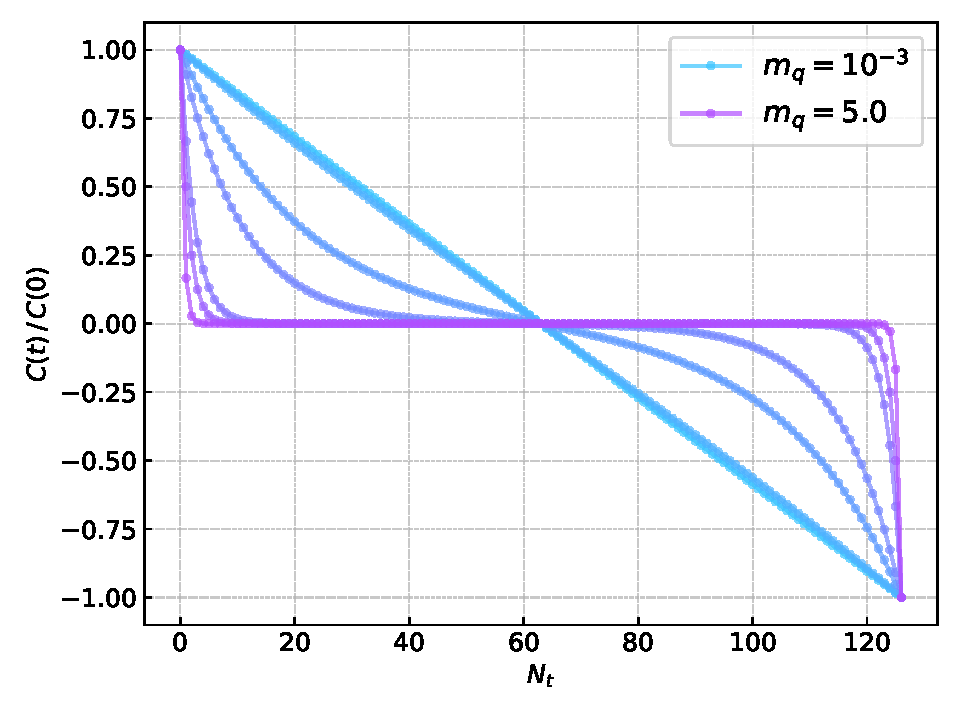
\includegraphics[scale=0.6]{figures/correlator/correlator.pdf}
    \caption[Fermionic correlator]{Normalised fermionic correlator for different values of the bare quark mass. A bigger mass results in a quicker decay, according to \textcolor{red}{eq. ref.}}
    \label{fig:correlator_mass}
\end{figure}
Figure \ref{fig:correlator_CGiter} shows the number of iterations needed for convergence of the Conjugate Gradient algorithm. While the exact number depends on the desired tolerance, one can clearly see that the number of iterations grows as $m_q \to 0$, due to an increase in the condition number \cite{cond_num_ref}. \\
\begin{figure}[h]
    \centering 
    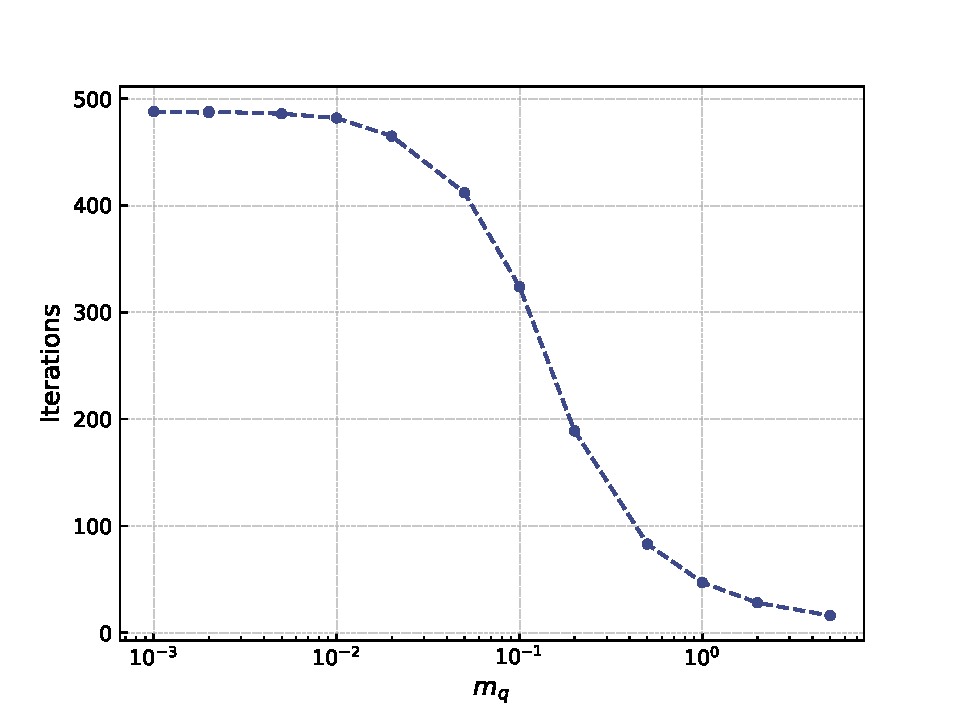
\includegraphics[scale=0.6]{figures/correlator/CGiter.pdf}
    \caption{CG iterations}
    \label{fig:correlator_CGiter}
\end{figure} 
\newpage
For the Dirac operator \textcolor{red}{ref eq.}, one can derive an analytical expression for the fermionic mass. The Dirac operator in momentum space reads \textcolor{red}{non lo hai mai introdotto}
\begin{equation*}
\bar{D}(p)= m_q + \sum_\mu 2 \sin ^2\left(\frac{p_\mu}{2}\right)+i \sum_\mu \gamma_\mu \sin \left(p_\mu\right)
\end{equation*}
and its inverse is
\begin{equation*}
    \bar{D}^{-1}(p) = \frac{m_q + \sum_\mu 2 \sin ^2\left(\frac{p_\mu}{2}\right) - i \sum_\mu \gamma_\mu \sin \left(p_\mu\right)}{m_q + \sum_\mu 2 \sin^2\left(\frac{p_\mu}{2}\right) + \sum_\mu \sin^2 \left(p_\mu\right)}.
\end{equation*}
One can now find the pole by imposing the numerator evaluated at $p^\mu =(im_\text{phys}, 0)$ to zero:
\begin{equation*}
    \left[m_q + \sum_\mu 2 \sin ^2\left(\frac{p_\mu}{2}\right)\right]^2_{p_\mu = (im_\text{phys}, 0)} + \left[\sum_\mu \gamma_\mu \sin \left(p_\mu\right)\right]^2_{p_\mu = (im_\text{phys}, 0)} = 0.
\end{equation*}
This results in a trascendental equation 
\begin{equation*}
    \left[m_q - 2 \sinh^2\left(\frac{m_\text{phys}}{2}\right)\right]^2 - \sinh^2\left(m_\text{phys}\right) = 0,
\end{equation*}
which has the solution 
\begin{equation}
    m_\text{phys} = \log\left(1+m_q\right).
    \label{eq:analytical_wilson}
\end{equation}
We then choose three values of the bare quark mass, compute the correlator numerically and perform a fit according to \eqref{eq:correlator_mass_extraction}, in order to extract the physical mass. We then compare it to the theoretical value given by \eqref{eq:analytical_wilson}. The results are reported in figures \ref{fig:fit_wilson} and table \ref{tab:free_wilson_fit}. \\~\\
\begin{table}
    \centering
    \begin{tabular}[pos]{ccc}
        \toprule
        $m_q$ & teo & fit \\
        \midrule 
        1.0 & 0.6931471805599453 & 0.6931537171644739 \\
        0.1 & 0.09531017980432493 & 0.09531020915059212 \\
        0.01 & 0.009950330853168092 & 0.009950277657505842 \\
        \bottomrule
    \end{tabular}
    \caption[Fit of the correlator for free Wilson fermions.]{The correlator for free Wilson fermions is fitted to \textcolor{red}{(eqref)} and compared to its analytical value given by \eqref{eq:analytical_wilson}. The precision for the Conjugate Gradient algorithm was set to $r^2 \leq 10^{-10}$.}
    \label{tab:free_wilson_fit}
\end{table}
\begin{figure}
    \centering
    \begin{subfigure}[b]{0.48\textwidth}
        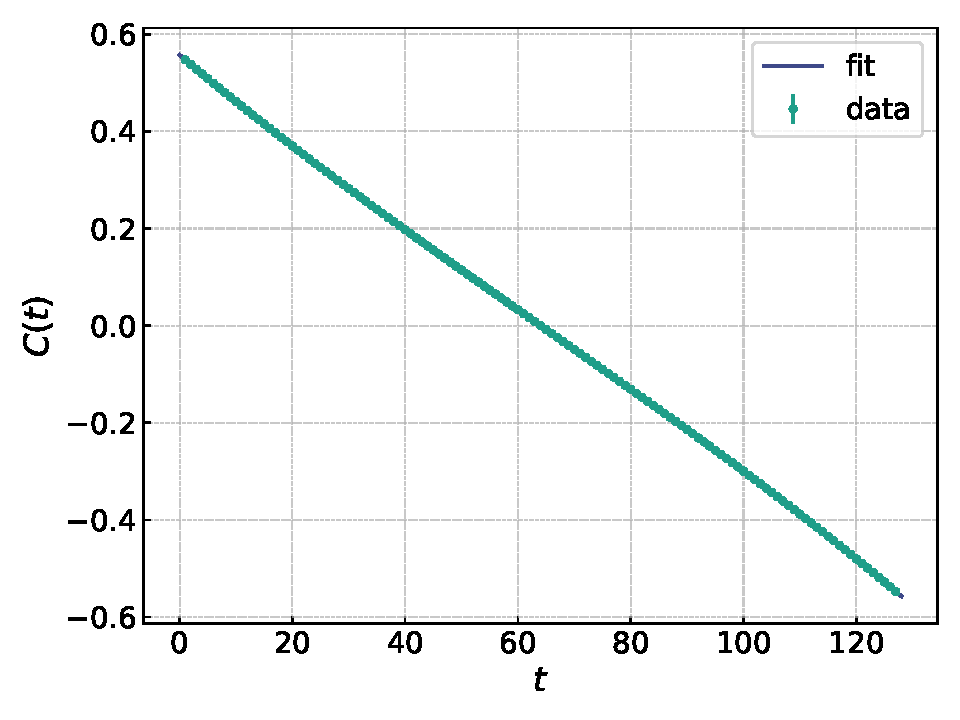
\includegraphics[width=1.05\textwidth]{figures/correlator/corrs_free/corr_small.pdf}
        \caption{$m_q = 0.01$}
    \end{subfigure}
    \hfill
    \begin{subfigure}[b]{0.48\textwidth}
        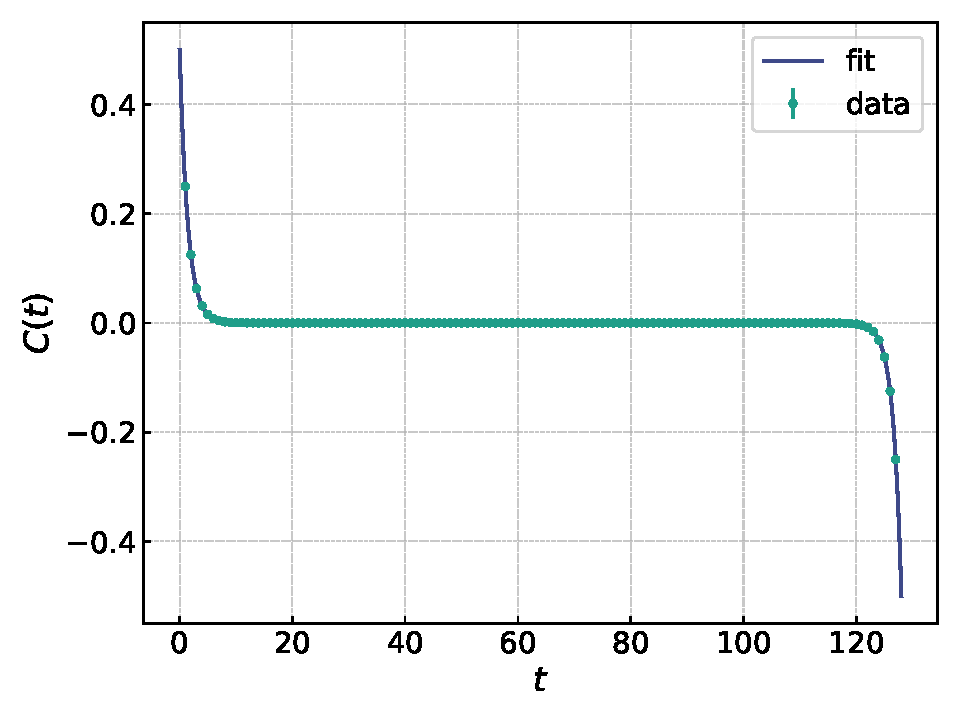
\includegraphics[width=1.05\textwidth]{figures/correlator/corrs_free/corr_big.pdf}
        \caption{$m_q = 1.0$}
    \end{subfigure}
    \\
    \vspace{10pt}
    \begin{subfigure}[b]{0.68\textwidth}
        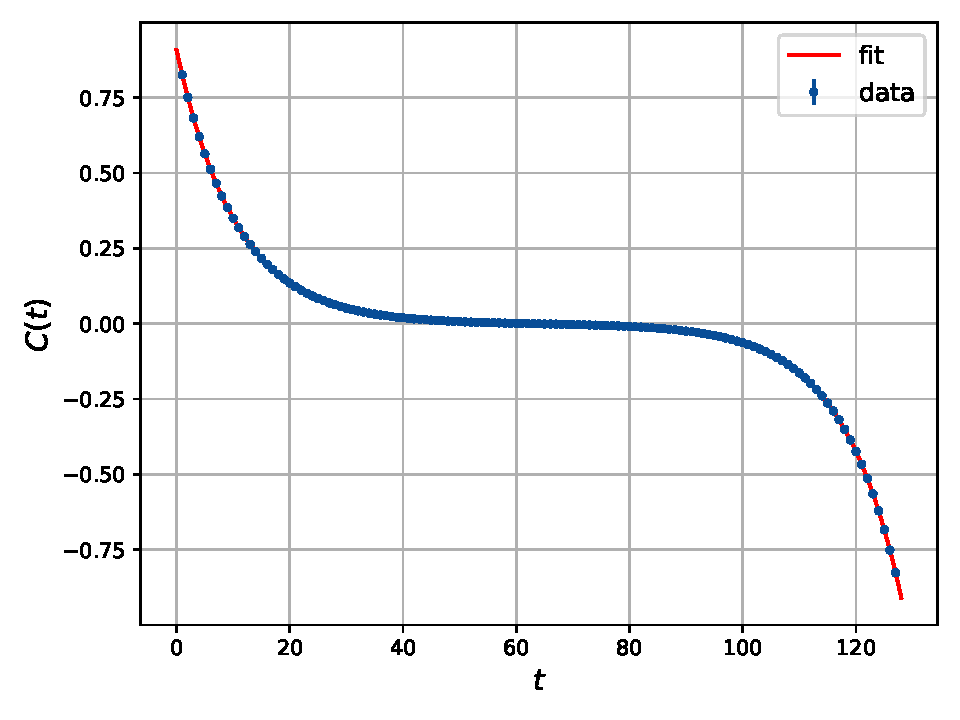
\includegraphics[width=1.05\textwidth]{figures/correlator/corrs_free/corr_medium.pdf}
        \caption{$m_q = 0.1$}        
    \end{subfigure}
    \caption[Fit of the correlator for free Wilson fermions.]{Fit of the fermionic correlator to \textcolor{red}{(eqref)}, for three different values of the bare quark mass.}
    \label{fig:fit_wilson}
\end{figure}
\textcolor{green}{The presence of a background field has the same effects on the correlator as a bare quark mass. In fact, if $\phi(x) = v$, one can simply redefine the bare mass as $M_q = m_q + g \, v$ and the properties of the fermionic correlator remain unchanged.}
\newpage

\section{Phase diagram}

We want to start the analysis of the Yukawa theory by doing a parameters scan, in order to have a global picture of the phase diagram in the presence of Wilson fermions.
\begin{figure}
    \centering
    \begin{subfigure}[b]{0.3\textwidth}
        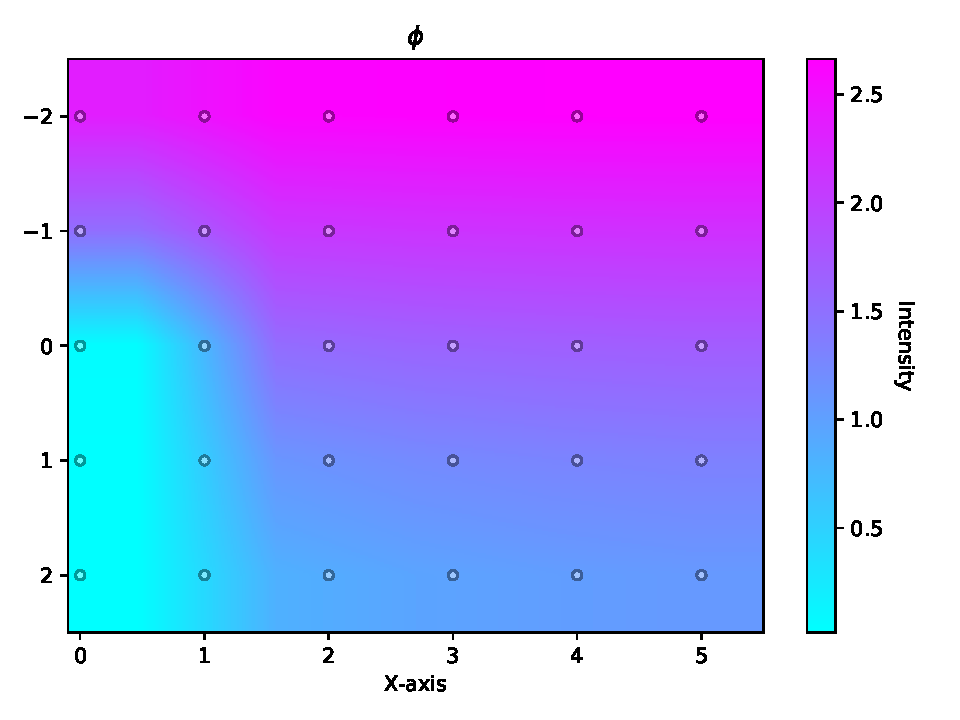
\includegraphics[width=\textwidth]{figures/phase_diagram/m_g_phi.pdf}
        \caption{$m_q = 1.0$}
    \end{subfigure}
    \begin{subfigure}[b]{0.3\textwidth}
        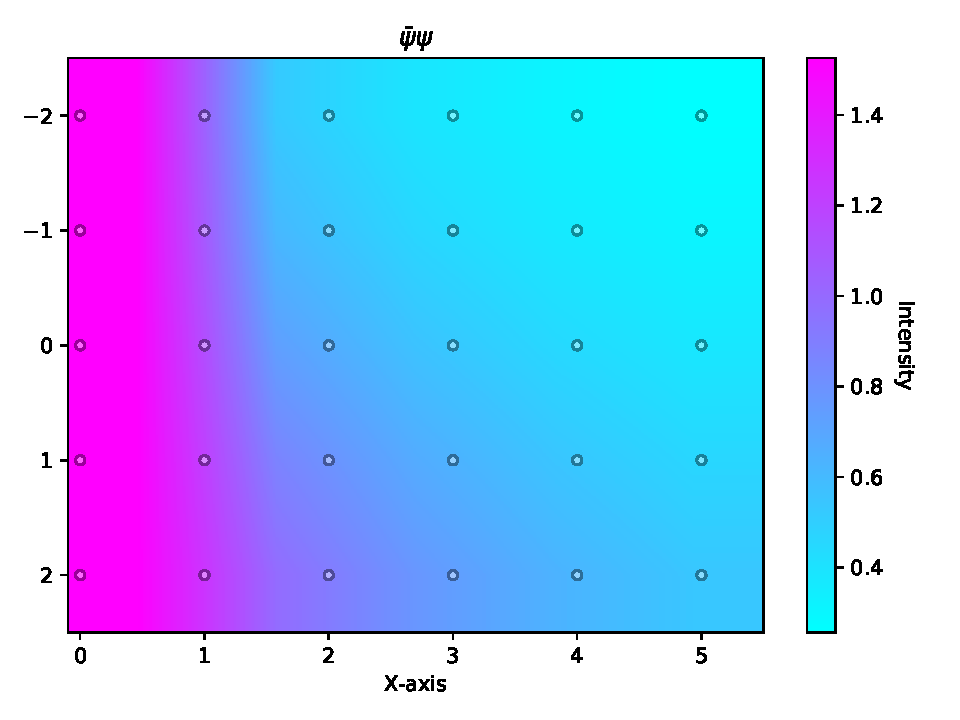
\includegraphics[width=\textwidth]{figures/phase_diagram/m_g_cond.pdf}
        \caption{$m_q = 1.0$}
    \end{subfigure}
    \begin{subfigure}[b]{0.3\textwidth}
        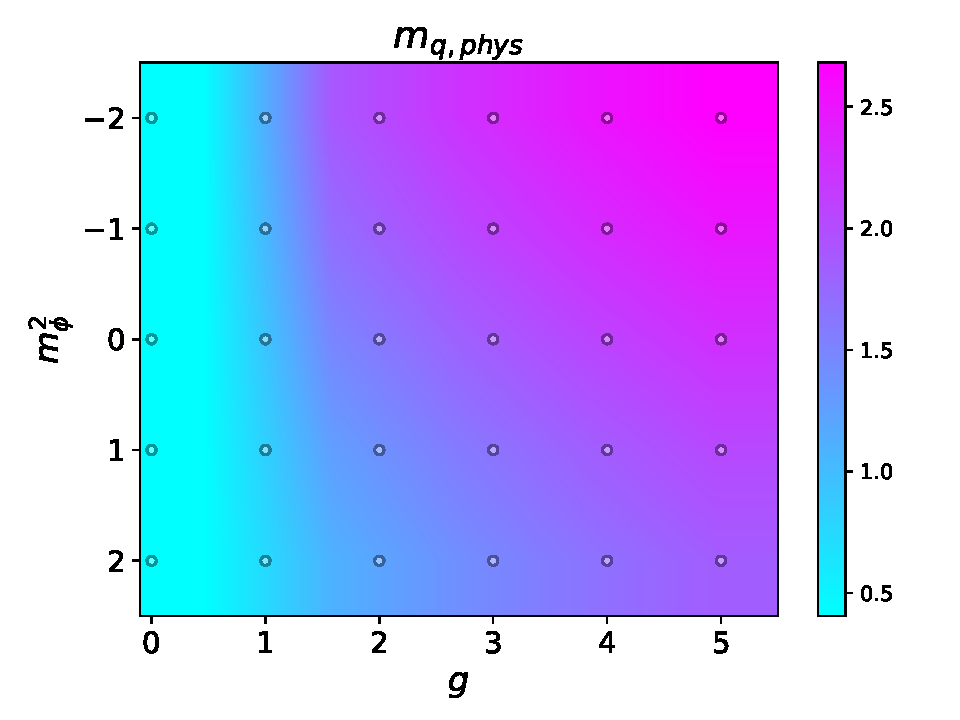
\includegraphics[width=\textwidth]{figures/phase_diagram/m_g_mq.pdf}
        \caption{$m_q = 1.0$}
    \end{subfigure}
    \begin{subfigure}[b]{0.3\textwidth}
        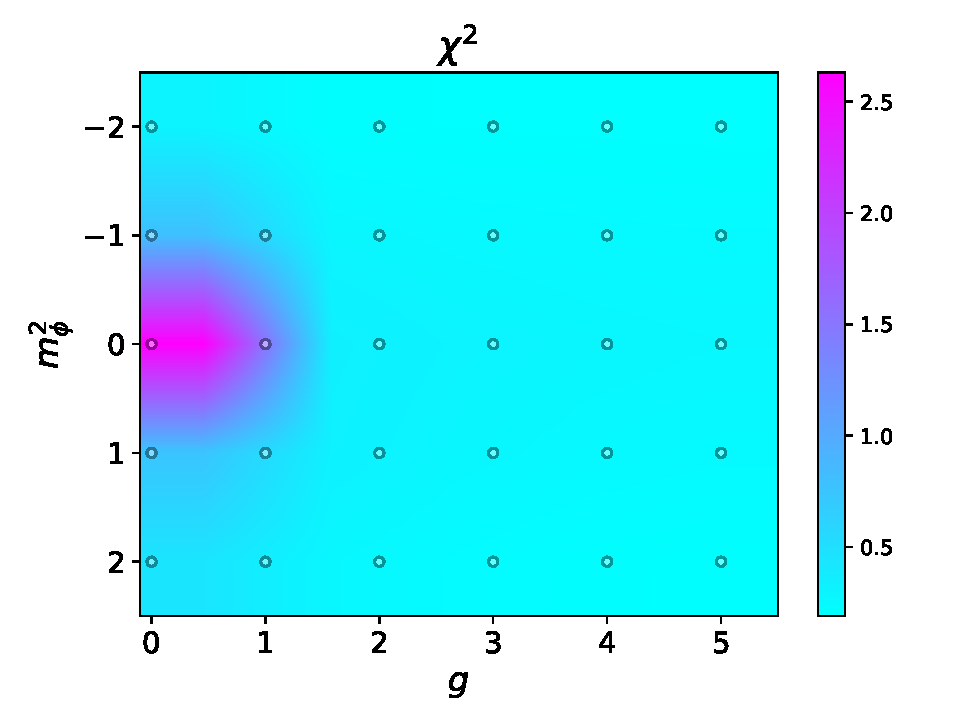
\includegraphics[width=\textwidth]{figures/phase_diagram/m_g_chi2.pdf}
        \caption{$m_q = 1.0$}
    \end{subfigure}
    \caption{Phase diagram - magnetisation}
    \label{fig:phase_diagram_phi}
\end{figure}

\chapter{Numerical results: coloured noise}
\label{chapt:results_coloured}

\section{Classical-to-quantum interpolation}

\label{sec:classical_to_quantum}

\begin{figure}[h]
    \centering
    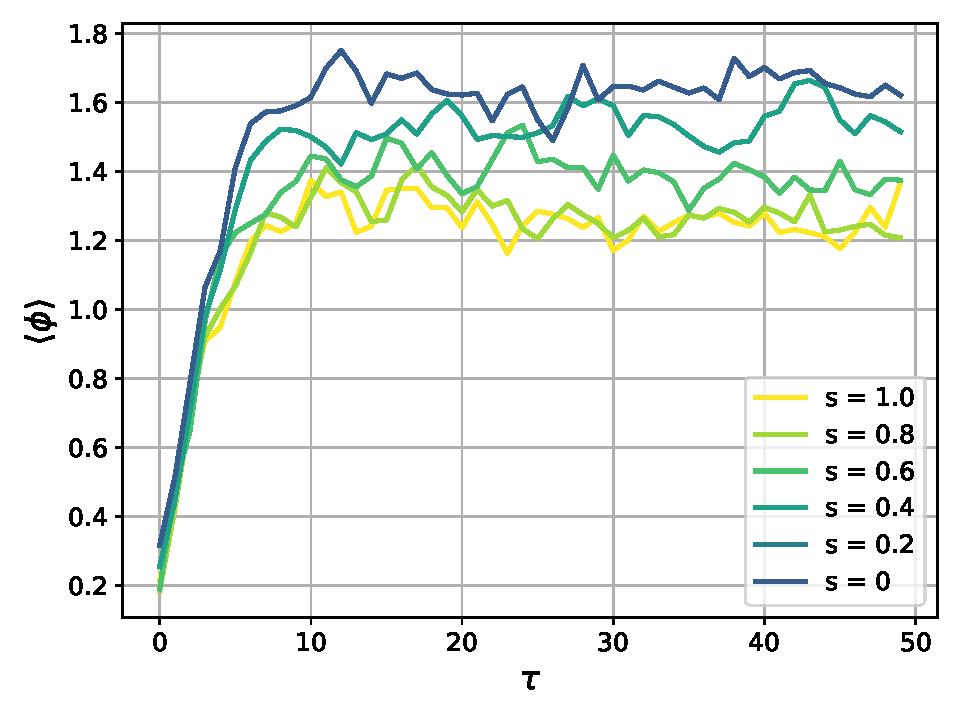
\includegraphics[width=0.8\textwidth]{figures/slide_broken/thermalisation.pdf}
    \caption[Thermalisation of the system for different values of the noise fraction $s$.]{Thermalisation of the system for different values of the noise fraction $s$. As noise is added, the equilibrium state of the system shifts accordingly. Coloured noise allows for a smooth interpolation between the fully classical and fully quantum picture.\\ $g=, \lambda=$, \dots}
    \label{fig:thermalisation_different_noise_fracs}
\end{figure}

Let us start by analising the coloured noise field in the simulation and relevant properties that emerge from it. We consider the Yukawa model described by the continuum action \eqref{eq:full_action_continuum} and its discrete version \eqref{eq:discretised_action}, \eqref{eq:discretised_effective_action}.\\
The system is initialised in the same state for all the configurations on a $64 \times 64$ lattice. We consider a simulation with $s=1$ and then progressively lower the cutoff fraction $s$, keeping fixed all the quantities in the classical action. \\
Figure \ref{fig:thermalisation_different_noise_fracs} shows the system thermalisation for different values of $s$, namely the Langevin evolution from the initial state to equilibrium. The blue line corresponds to the case $s=0$, a classical simulation, while the brown line corresponds to the case $s=1$, the fully quantum case.  All the parameters settings are reported under the figure. \\
One can notice that as quantum modes are removed via coloured noise, the systems shifts its equilibrium point. \\~\\ 
We now want to study observable values at equilibrium, as a function of the noise fraction $s$. In particular it is of our interest to investigate the interplay relation among the field $\phi$, the chiral condensate $\bar\psi\psi$ and the quark mass $m_\text{phys}$, which was discussed in section \ref{sec:Yukawa_theory}.
\begin{equation*}
	\expect{\phi} \sim \expect{\bar\psi\psi} \sim m_q.
\end{equation*}
For $s=0$, the fields are restricted to the classical equations of motion \eqref{eq:classical_EOM_full}. As pointed out in section \ref{sec:Yukawa_theory}, in particular in equation \eqref{eq:background_field}, a background field $\phi(x) = v$ has the same behaviour on the system as a bare quark mass. We then compare the physical quark mass with the theoretical expression for free Wilson fermions \eqref{eq:analytical_wilson} using a shifted bare mass 
\begin{equation*}
	M_q = m_q + g \expect{\phi}
\end{equation*}
The comparison is reported in table \ref{tab:background_field}
\begin{table}[htp]
    \centering
    \begin{tabular}{cccccc}
        \toprule
        $m_q$ & $g$ & $\expect{\phi}$ & $M_q$ & $\log(1+M_q)$ & $m_\text{phys}$ \\
        \midrule
	$1.0$ & $0.2$ & 3.032082758 & 1.606416551
    & 0.957976309
    & 0.957976383 \\
        \bottomrule
    \end{tabular}
    \caption[Background field and quark mass]{The physical quark mass of the classical system is compared with the theoretical result for Wilson fermions, using the shifted bare mass $M_q = m_q + g \left\langle\phi\right\rangle$. This shows that a background scalar field can be interpreted as a bare quark mass.}
    \label{tab:background_field}
\end{table}
\begin{figure}
    \centering
    \begin{subfigure}[b]{0.48\textwidth}
        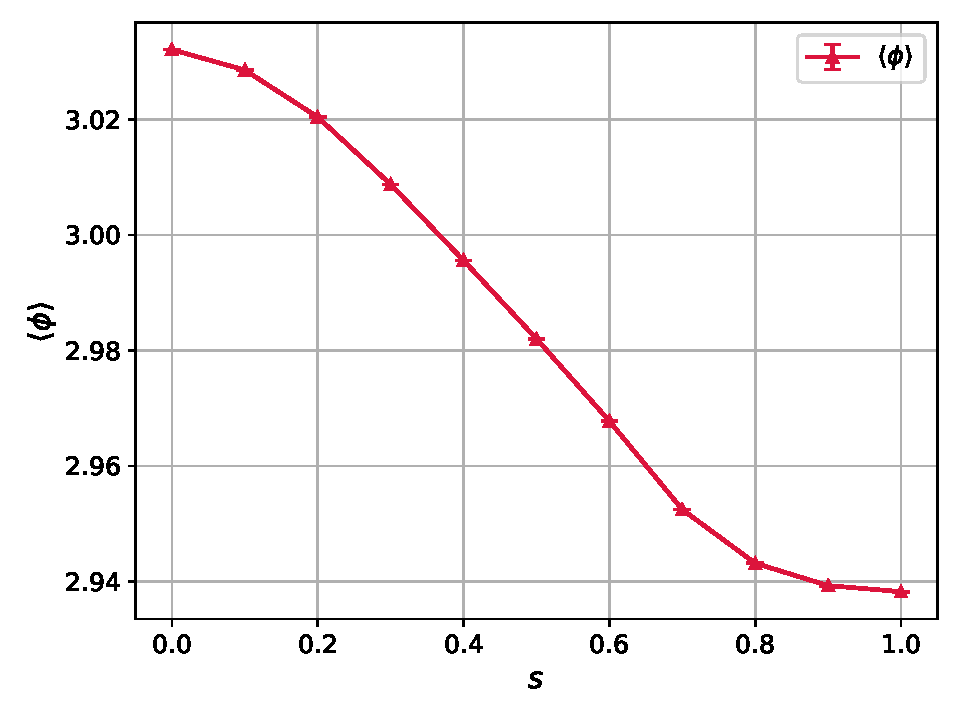
\includegraphics[width=1.0\textwidth]{figures/slide_broken/magnetisation.pdf}
    \end{subfigure}
    \begin{subfigure}[b]{0.48\textwidth}
        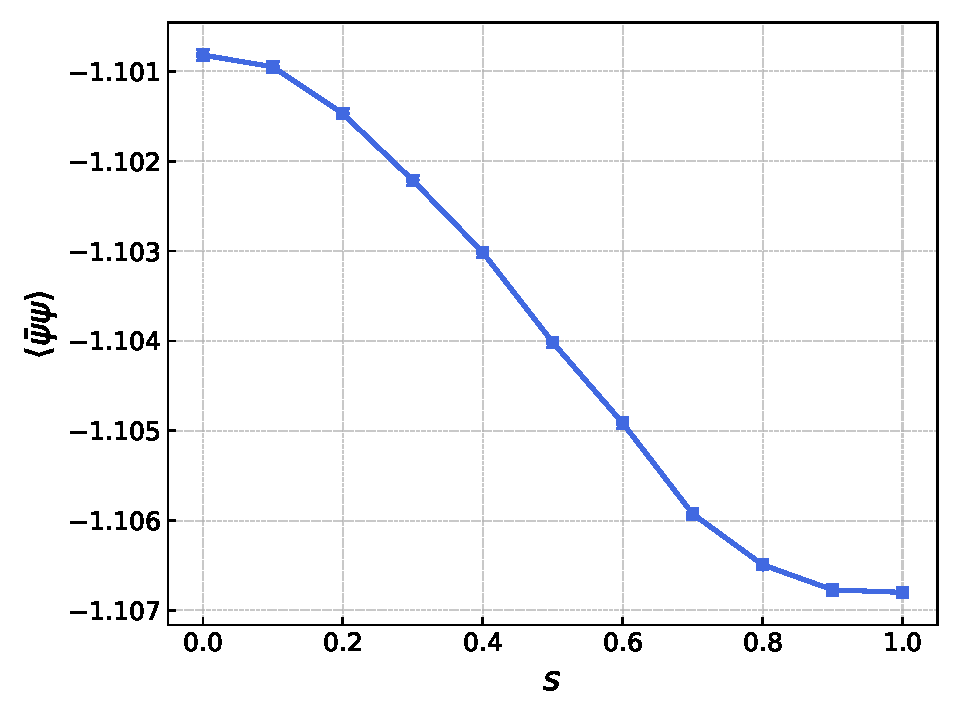
\includegraphics[width=1.0\textwidth]{figures/slide_broken/condensate.pdf}
    \end{subfigure}
    \begin{subfigure}[b]{0.48\textwidth}
        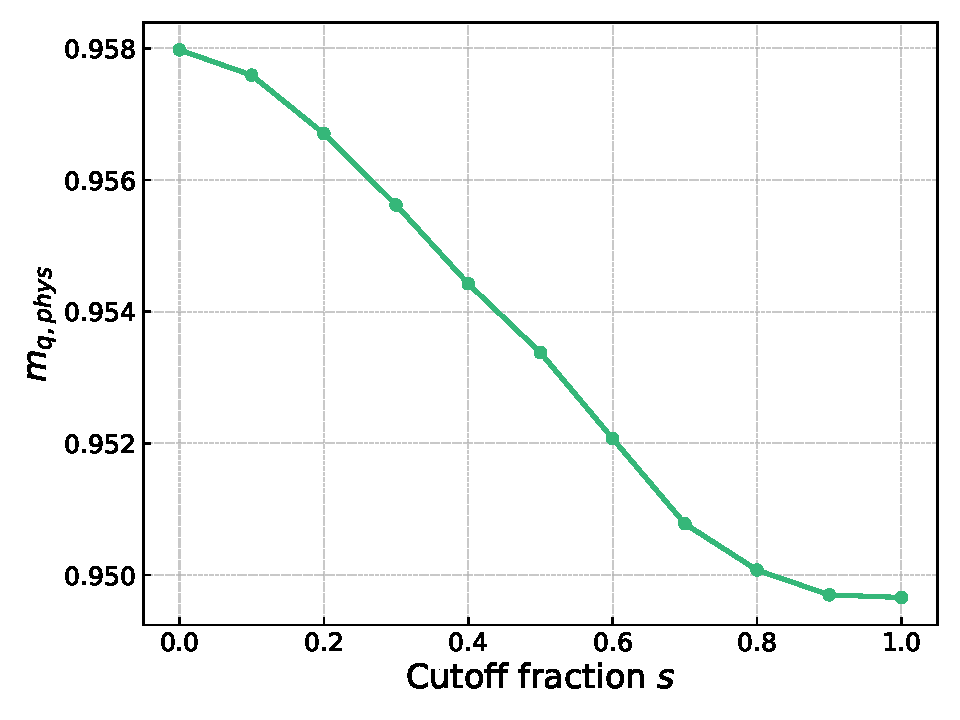
\includegraphics[width=1.0\textwidth]{figures/slide_broken/mass.pdf}
    \end{subfigure}
    \caption[Relation between magnetisation, condensate and mass]{Qualitative relation between magnetisation, chiral condensate and mass, which was motivated in section \ref{sec:Yukawa_theory}. The parameters settings for the configuration are $m_\phi^2=, \lambda=, m_q=, g=$}
    \label{fig:interpolation_relation_phi_cond_mass}
\end{figure}
\newpage


\section{Chiral fermions and noise-induced chiral phase transition}
\label{sec:chiral_PT}
\textcolor{red}{comment on the configurations}
As explained in section \ref{sec:Yukawa_theory}, chiral symmetry can be broken, in the continumm theory, either explicitly via the introduction of a finite bare quark mass, or spontaneously if the field gains a non-zero expectation value.\\
Moreoveor, in the discrete formulation, the introduction of the Wilson term contributes to the explicit breaking of chiral symmetry, as shown in appendix \ref{chap:AppendixB}. This, in particular, means that chiral symmetry is explicitly broken also for $m_q \to 0$. Because of this, one needs a new definition of the bare mass $M_q$, which takes into account the Wilson term contribution, such that chiral symmetry is restored in the limit $M_q \to 0$. \\
In a lattice study of a theory suchs as  two-flavours QCD, what one typically does \cite{rothe_LGT,gattringer_LQCD} is the following: the spontaneous breaking of chiral symmetry generates three goldstone massless bosons, the pions. If the bare quark mass is zero, the physical mass of the pions has to be zero, as a consequence of Goldstone's theorem \cite{goldstone}. Hence one can measure the pions mass and find a value $m_q^*$ such that when $m_q \to m_q^*$ one has $M_\pi \to 0$. \\
This approach is not feasible in our theory, since it is described by a discrete chiral symmetry. \\
In the literature, one can find proposals for the definition of a bare quark mass for similar theories \cite{Iwasaki:1994gq,MAIANI1986265}. Thus such approaches are not followed here, both because of time reasons, but also because it is not our purpose to match any physical results, but rather investigate properties of the coloured noise technique. Hence, here we just consider na\"ive fermions and the chiral limit is reached for $m_q \to 0$. Thus, one has to keep in mind that due to the fermion doubling, this represents a theory with $2N_f = 4$ physical degenerate quarks. \\~\\
\begin{figure}[h]
    \centering
    \captionsetup[subfigure]{justification=centering}
    \begin{subfigure}[t]{0.48\textwidth}
        \centering
        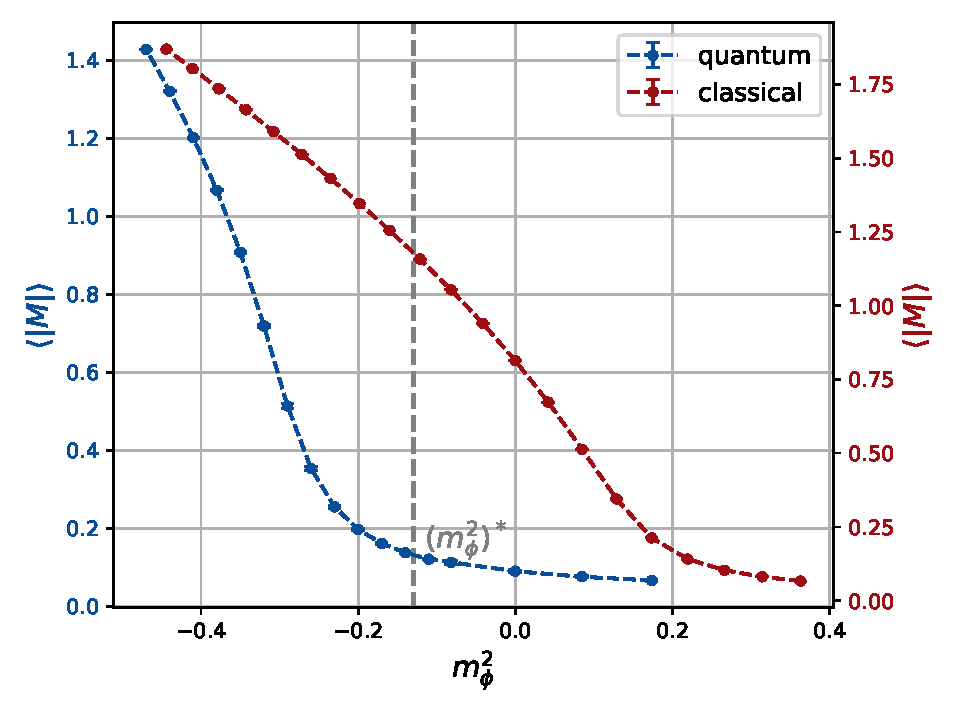
\includegraphics[width=1.05\textwidth]{figures/chiral_PT/mass_scan/magnetisation.pdf}
    \end{subfigure}
    \hfill
    \begin{subfigure}[t]{0.48\textwidth}
        \centering
        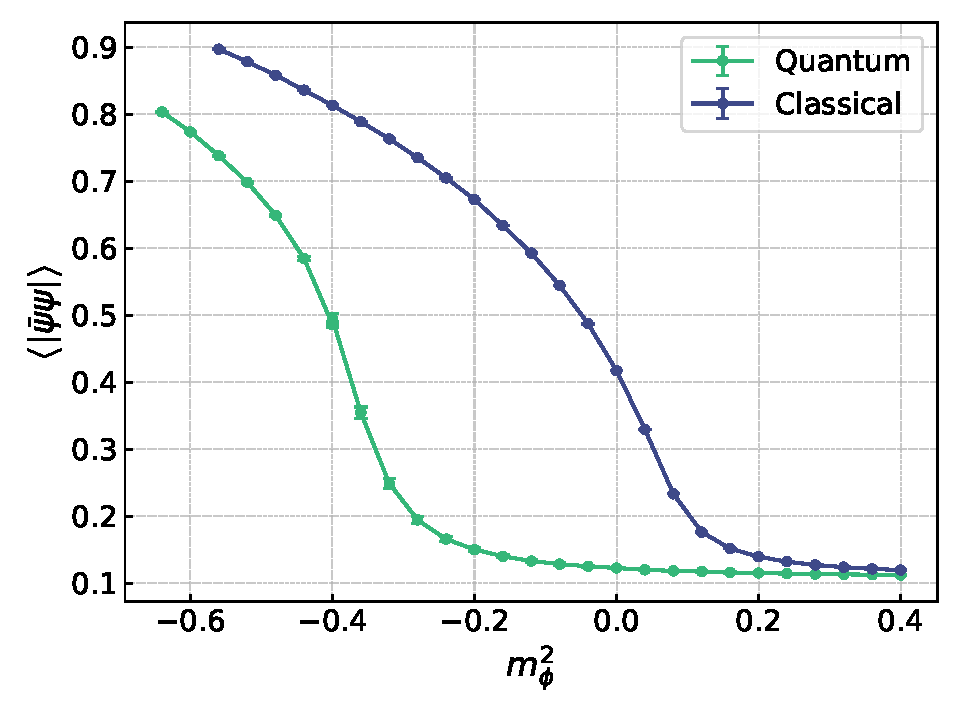
\includegraphics[width=1.05\textwidth]{figures/chiral_PT/mass_scan/condensate.pdf}
    \end{subfigure}
    \caption[Mass scan of the quantum and classical theories]{Mass scan of the quantum and classical theories. The dashed gray line indicates a value $m_\phi^{2, \,*}$, where the classical and quantum systems lie in two different phases.}
    \label{fig:scans_classical_quantum}
\end{figure} 
In figure \ref{fig:scans_classical_quantum}, the (absolute) magnetisation and the chiral condensate are studied as a function of the bosonic mass squared, both in the fully quantum and fully classical theory. One can notice that the classical system undergoes a phase transition at values of $m_\phi^2$ bigger than the quantum counterpart. Note that as the bare quark mass is small but finite, this is not a proper phase transition and the latter will be, eventually, reached in the limit $m_q \to 0$. We then pick a value $m_\phi^{2 \, *} = -0.123$ which is represented by a gray line in figure \ref{fig:scans_classical_quantum}.
Using coloured noise, we then interpolate between the classical and quantum picture for different values of the quark mass, namely $m_q = 10^{-2}, 5 \cdot 10^{-3}, 10^{-3}$.
\begin{figure}[h]
\centering
\begin{minipage}{0.45\textwidth}	
	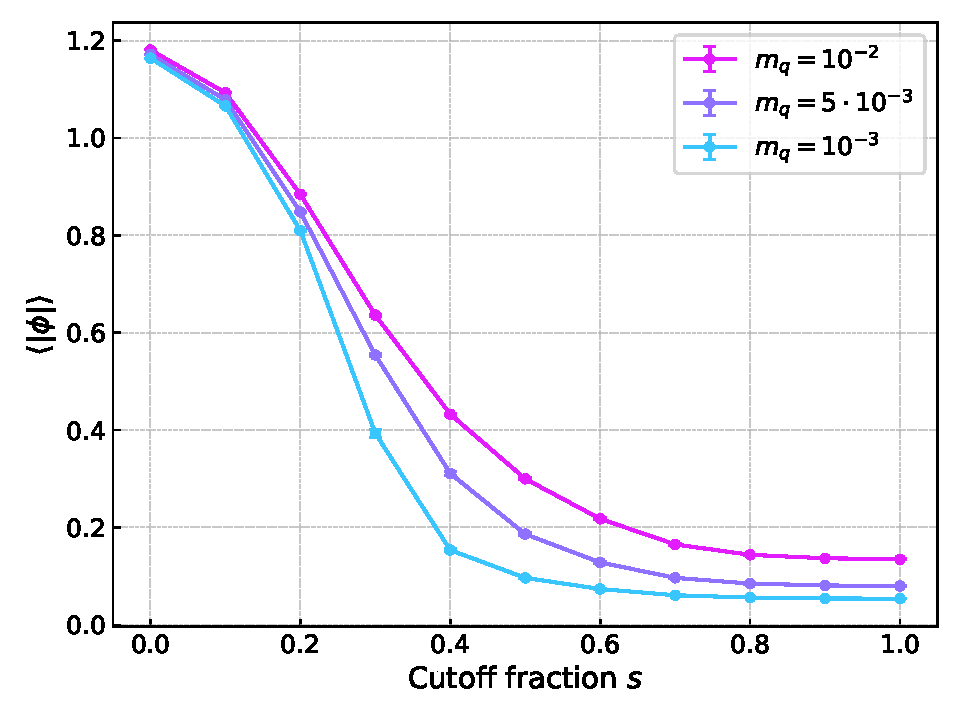
\includegraphics[scale=0.48]{figures/chiral_PT/magnetisation.pdf}
\end{minipage}
\hfill
\begin{minipage}{0.45\textwidth}	
	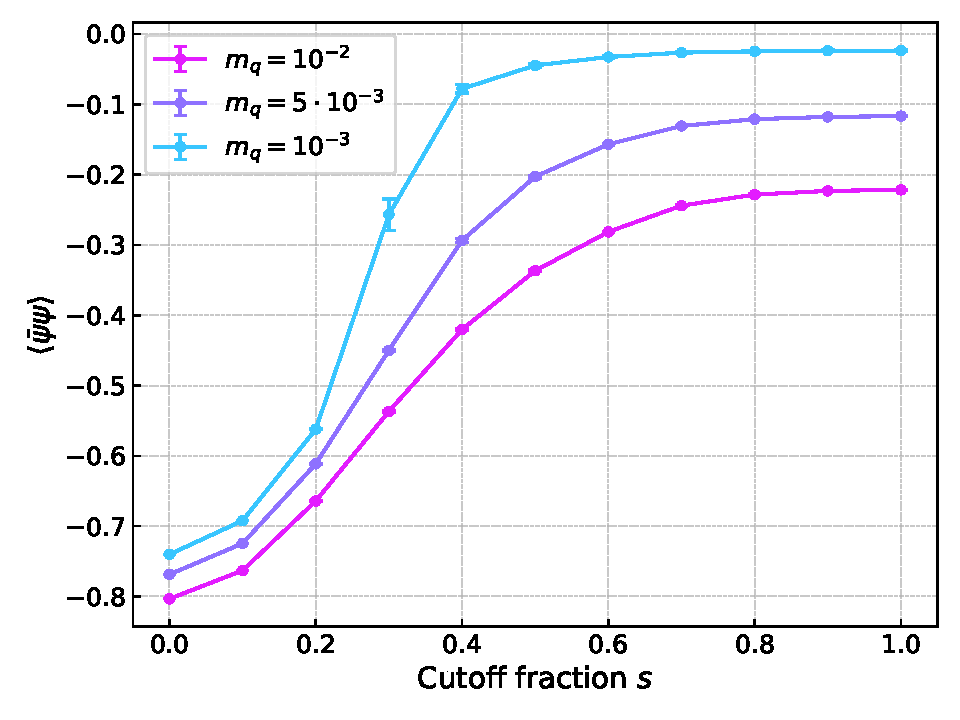
\includegraphics[scale=0.48]{figures/chiral_PT/condensate.pdf}
\end{minipage}
\begin{minipage}{0.45\textwidth}	
	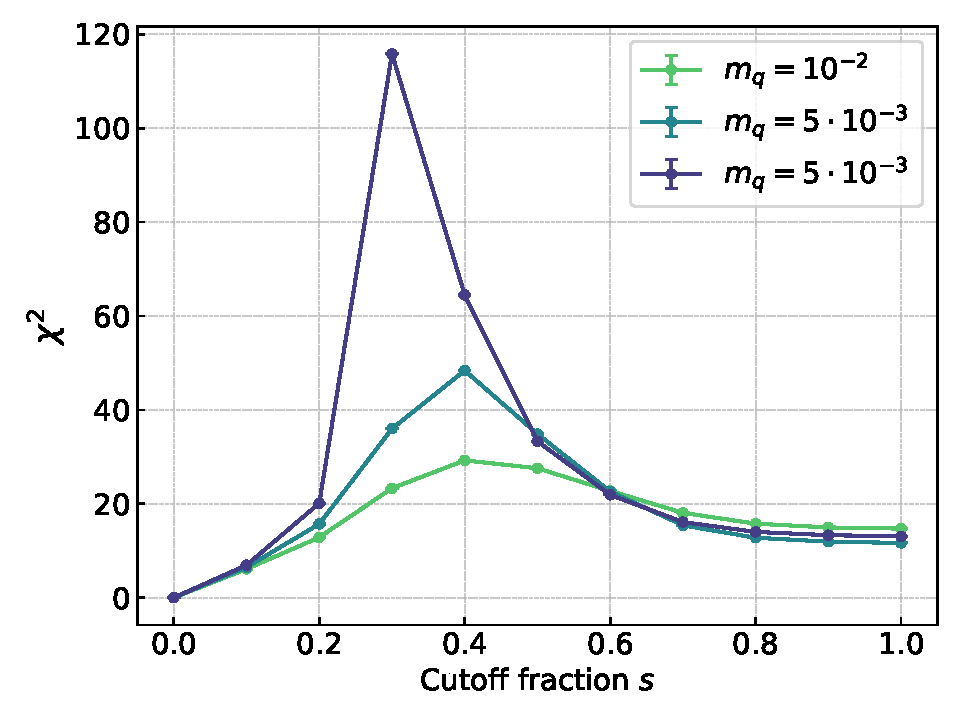
\includegraphics[scale=0.48]{figures/chiral_PT/chi2.pdf}
\end{minipage}
\hfill
\begin{minipage}{0.45\textwidth}
	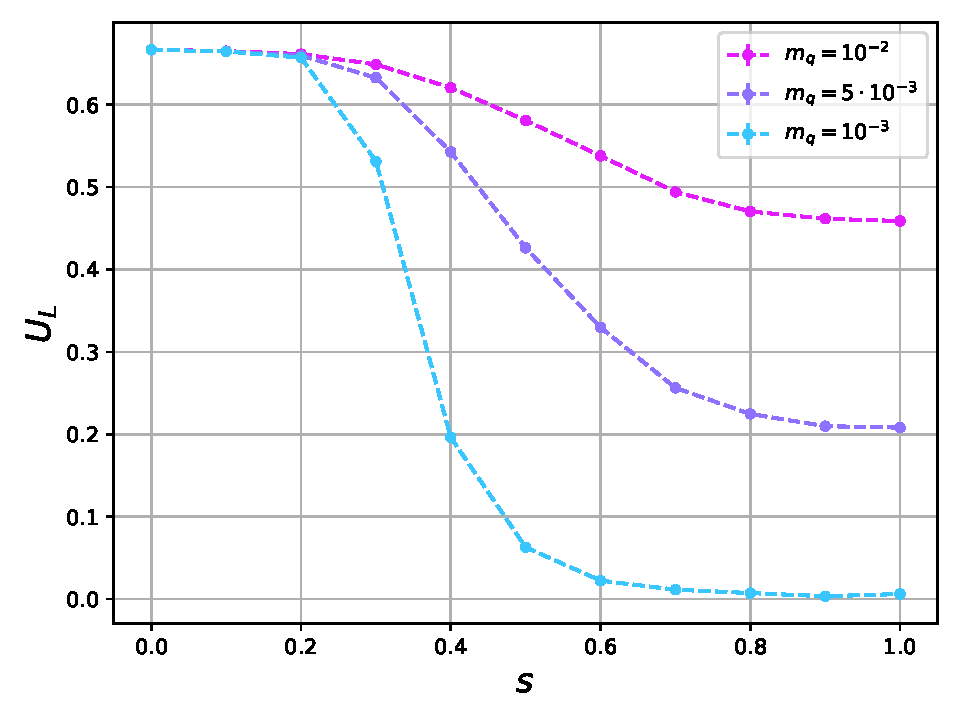
\includegraphics[scale=0.48]{figures/chiral_PT/binder.pdf}
\end{minipage}
\hfill
\caption{Noise-induced chiral phase transition}
\label{fig:chiral:symmetry_breaking}
\end{figure}\\
One can clearly see in figure \ref{fig:chiral:symmetry_breaking} that as the quark  mass is lowered the difference between the two phases gets sharper, indicating a phase transition. 
This is especially highligthed in the increasing peak of the magnetic susceptibility, and by the Binder parameters, which is supposed to assume the vlaue $U_L = 0$ in the symmetric phase, and $U_L=2/3$ in the broken phase.
\newpage

\section{Cooling with coloured noise}
Let us now consider one of the main applications of coloured noise, namely the cooling technique. \\
We first set up a white noise simulation $s=1$, and then progressively lower $s$. The lowering of the cutoff is compensated by a change in the couplings, as explained in section  \ref{sec:lattice_with_coloured_noise}. A symmary of the parameters choice is reported in figure  \ref{tab:params_cooling}. \\
\begin{table}[htp]
    \centering
    \begin{tabular}{cccccccc}
        \toprule
        $s$ & $N_t$ & $N_x$ & $m_\phi^2$ & $\lambda$ & $g$ & $m_q$& $K_\psi$ \\
        \midrule 
        1 & 16 & 16 & $m_\phi^2$ & 0.4 & 0.3 & $0.5$ & $K_\psi$ \\
        1/2 & 32 & 32 & $m_\phi^2/4$ & 0.1 & 0.3 & $0.5$ & $K_\psi/4$ \\
        1/4 & 64 & 64 & $m_\phi^2/16$ & 0.025 & 0.3 & $0.5$ & $K_\psi/16$ \\
        1/8 & 128 & 128 & $m_\phi^2/64$ & 0.00625 & 0.3 & $0.5$ & $K_\psi/64$ \\
        \bottomrule
    \end{tabular}
    \caption[Parameters cooling]{Parameters setting in the cooling procedure. Each coupling in the bosonic action is rescaled according to its canonical dimension, while the fermionic sector rescaling is implemented directly at the drift level, as detailed in section \ref{sec:lattice_with_coloured_noise}}.
    \label{tab:params_cooling}
\end{table}
Figure \ref{fig:cooling_M_psibarpsi_chi2} reports the magnetisation, its susceptibility and the chiral condensate as a function of the bare scalar mass squared $m_\phi^2$.
\begin{figure}[hbp]
    \centering
    \begin{subfigure}[b]{0.48\textwidth}
        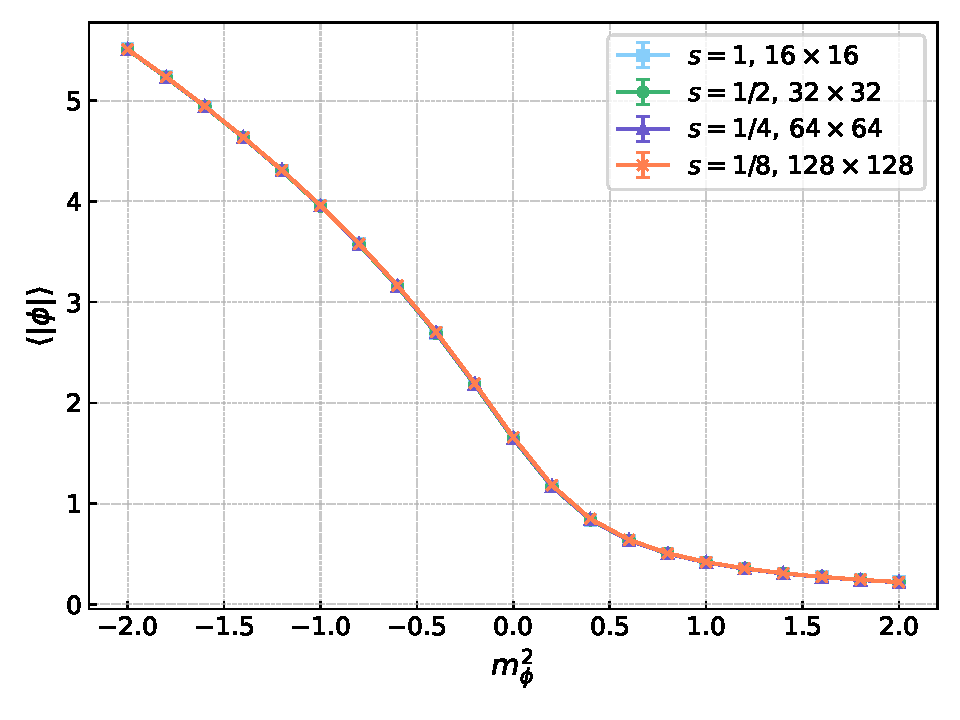
\includegraphics[width=1.05\textwidth]{figures/cooling/mass_scan/magnetisation.pdf}
    \end{subfigure}
    \hfill
    \begin{subfigure}[b]{0.48\textwidth}
        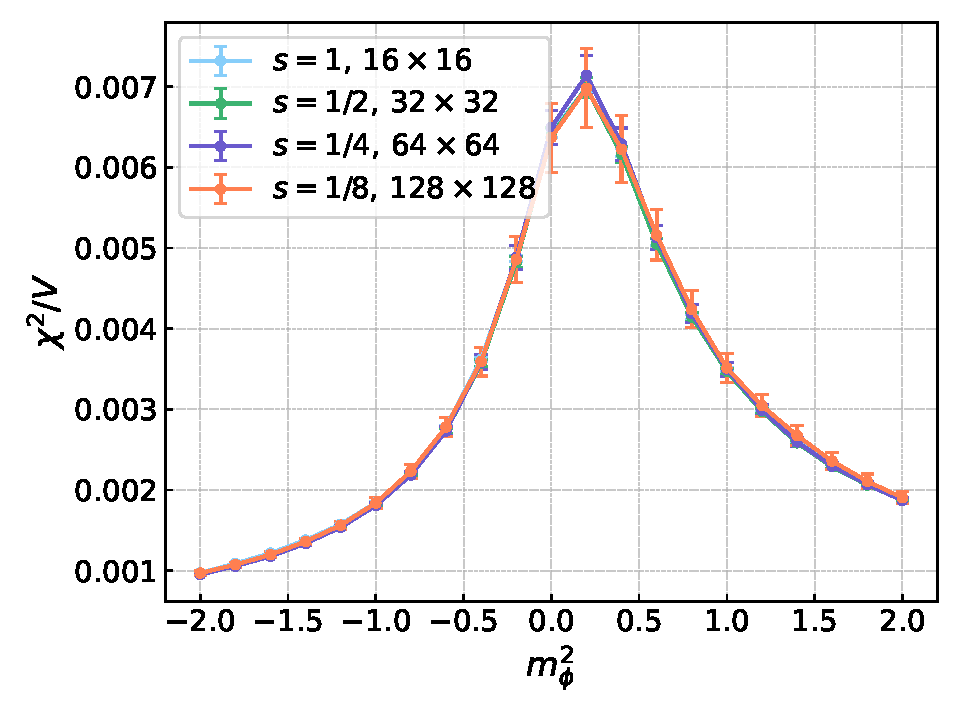
\includegraphics[width=1.05\textwidth]{figures/cooling/mass_scan/susceptibility.pdf}
    \end{subfigure}
    \\
    \vspace{10pt}
    \begin{subfigure}[b]{0.48\textwidth}
        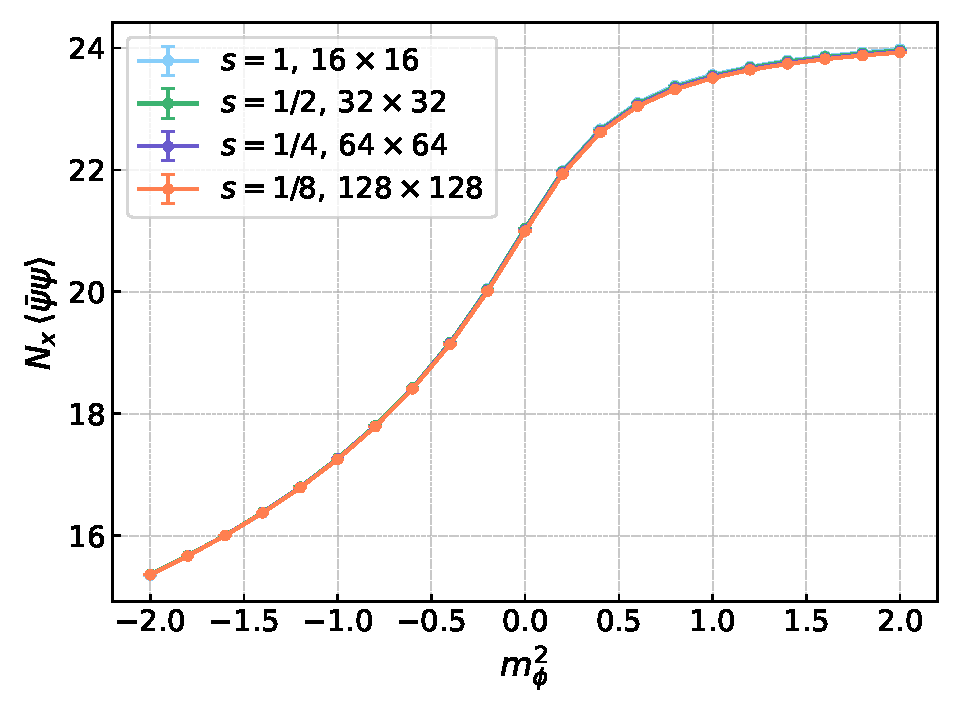
\includegraphics[width=1.05\textwidth]{figures/cooling/mass_scan/condensate.pdf}
    \end{subfigure}
    \caption[Cooling stochastic quantisation: fields as a function of the bosonic mass squared.]{Cooling via coloured noise. The absolute magnetisation, its susceptibility and the chiral condensate are compared after performing block-spins transformations. \\ $g = \dots$}
\end{figure}\\
A quantitative comparison for the magnetisation is reported in figure \ref{fig:cooling_deviation}, where we show the relative errors
\begin{equation}
    \begin{aligned}
        \epsilon_\phi(s) &= \frac{\expect{|M|}_{s} - \expect{|M|}}{\expect{|M|}}, \\
        \epsilon_\psi(s) &= \frac{\expect{|\bar\psi \, \psi|}_{s} - \expect{|\bar\psi \, \psi||}}{\expect{|\bar\psi \, \psi||}}.
    \end{aligned}
    \label{eq:cooling_relative_deviation}
\end{equation}
\begin{figure}[htp]
    \centering
    \begin{subfigure}[b]{0.48\textwidth}
        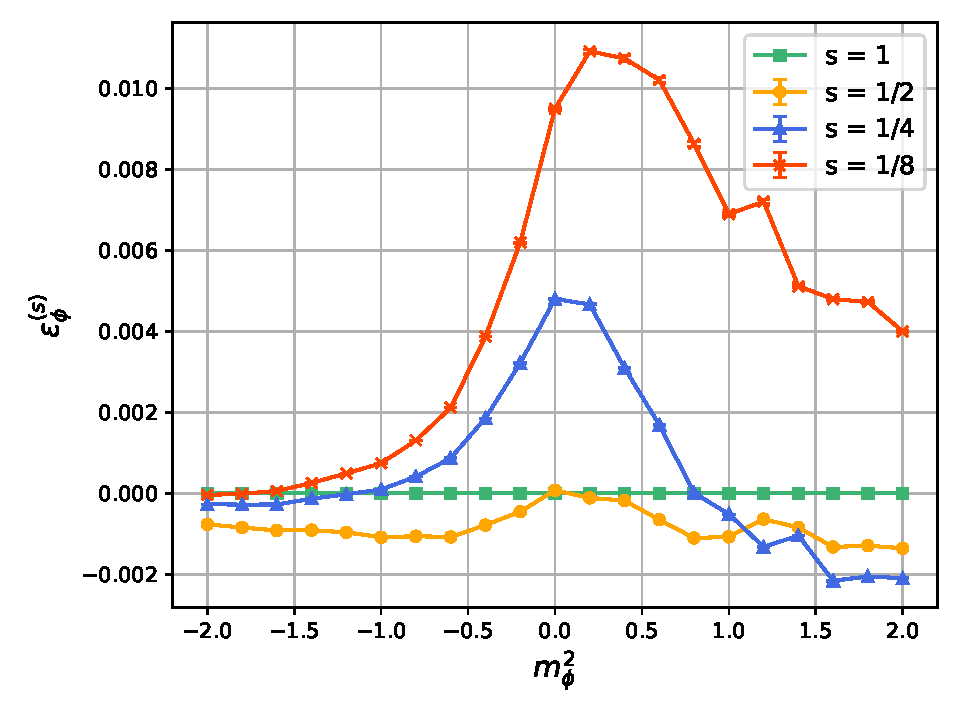
\includegraphics[width=1.0\textwidth]{figures/cooling/mass_scan/deviation.pdf}
        \caption{Absolute magnetisation}
    \end{subfigure}
    \begin{subfigure}[b]{0.48\textwidth}
        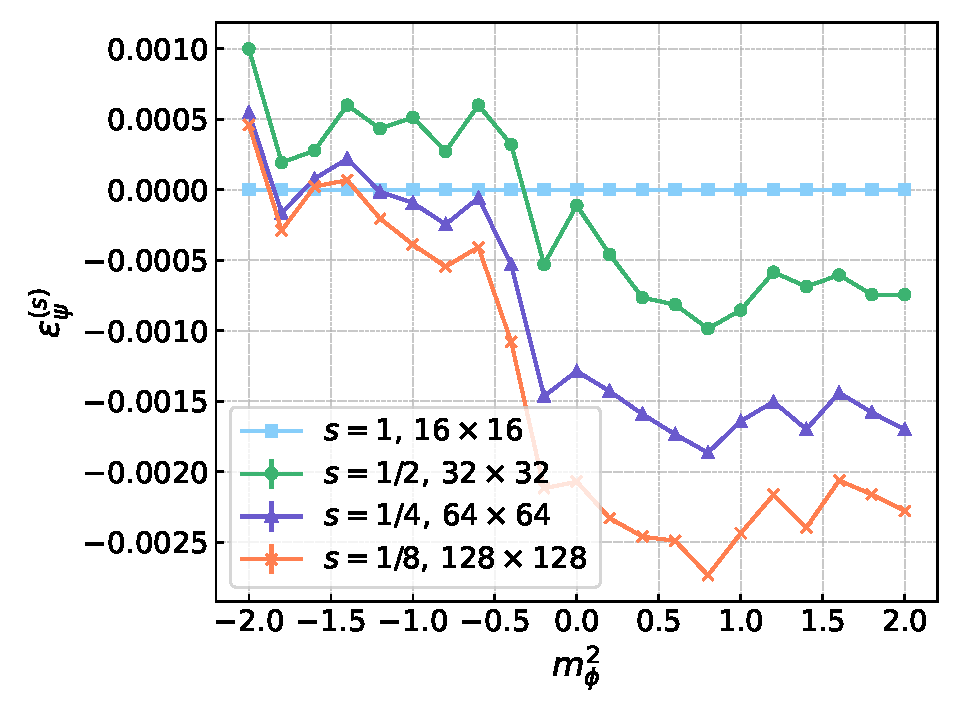
\includegraphics[width=1.0\textwidth]{figures/cooling/mass_scan/deviation_cond.pdf}
        \caption{Chiral condensate}
    \end{subfigure}
    \caption[Relative error in the cooling procedure at tree level.]{Relative error of the absolute magnetisation and chiral condensate in the cooling procedure for various values of the noise fraction $s$.}
    \label{fig:cooling_deviation}
\end{figure}\\
We also want to give a look at more complex observables such as the fermionic physical mass and the bosonic renormalised mass. They are reported in figure \ref{fig:cooling_masses}. As one can see, there is a clear deviation for $m_{\phi, r}$ at the third block-spin iteration. This is a systematic deviation because \textcolor{red}{i would say tree level, but I don't think it's the case.}
\begin{figure}[hbp]
    \begin{minipage}{0.45\textwidth}
        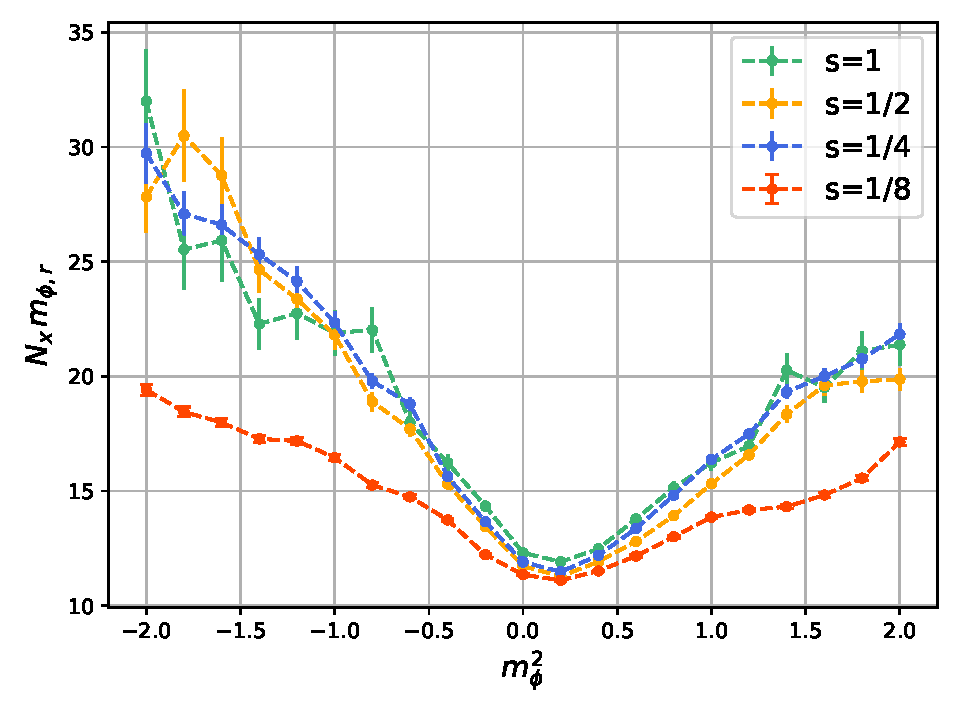
\includegraphics[scale=0.45]{figures/cooling/mass_scan/mphir.pdf}
    \end{minipage}
    \hfill 
    \begin{minipage}{0.45\textwidth}
        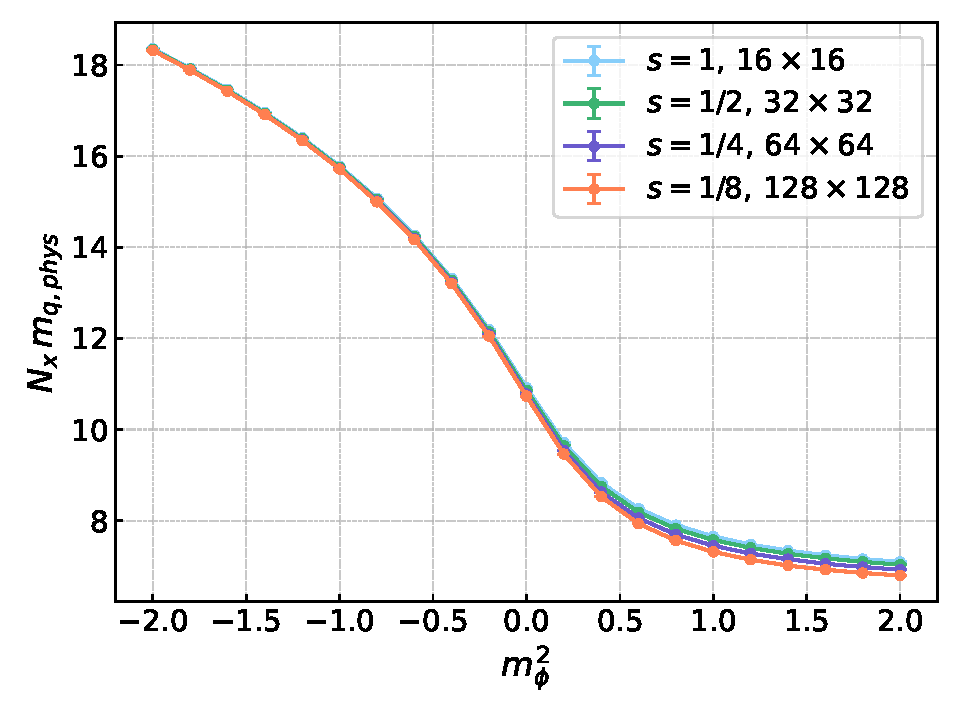
\includegraphics[scale=0.45]{figures/cooling/mass_scan/mqphys.pdf}
    \end{minipage}
    \caption[Masses in the cooling procedure]{Renormalised bosonic mass $m_{\phi, r}$ and pole fermionic mass $m_{q,\text{phys}}$ for various values of the noise fraction $s$.}
    \label{fig:cooling_masses}
\end{figure} \\
Finally, we report also the results for the magnetisation and the chiral condensate as a function of the Yukawa coupling.
\begin{figure}[hbp]
    \centering
    \begin{subfigure}[b]{0.48\textwidth}
        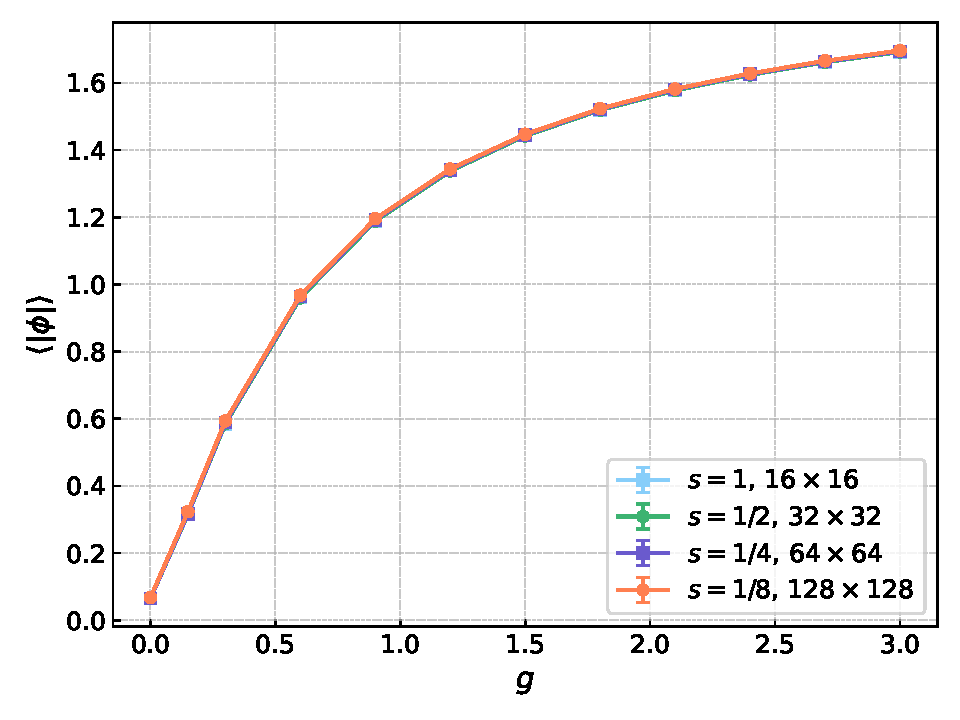
\includegraphics[width=1.05\textwidth]{figures/cooling/yukawa_scan/magnetisation.pdf}
        \caption{Magnetisation}
    \end{subfigure}
    \hfill
    \begin{subfigure}[b]{0.48\textwidth}
        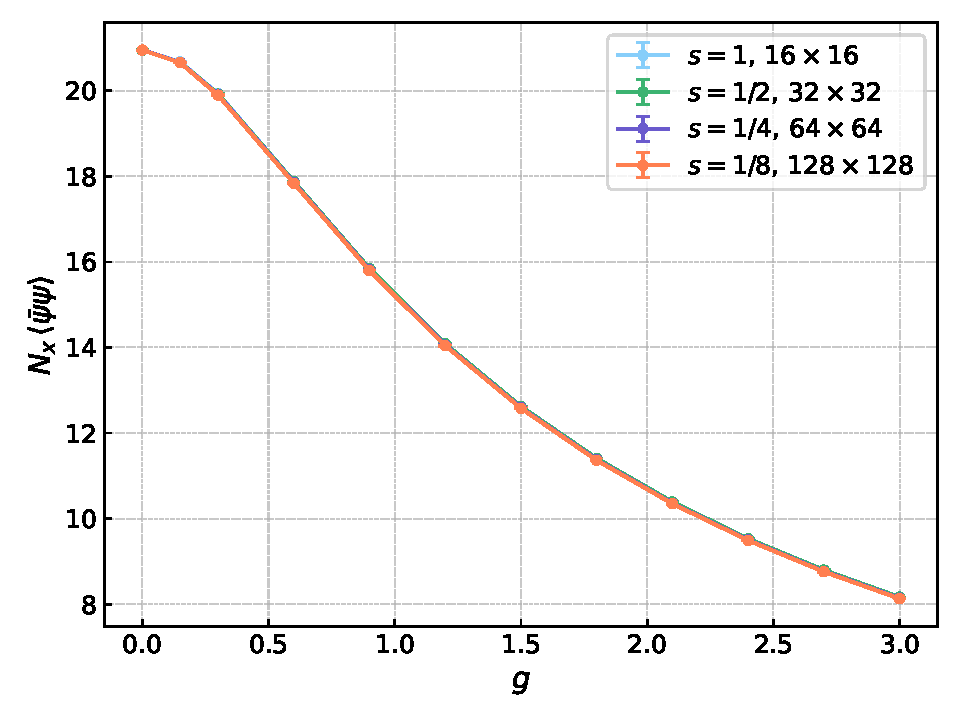
\includegraphics[width=1.05\textwidth]{figures/cooling/yukawa_scan/condensate.pdf}
        \caption{Chiral condensate}
    \end{subfigure}
    \caption[Cooling stochastic quantisation: fields as a function of the Yukawa coupling.]{Cooling via coloured noise. The absolute magnetisation and the chiral condensate are compared after performing block-spins transformations. \\ $g = \dots$}
    \label{fig:cooling_M_psibarpsi}
\end{figure}
\begin{figure}[htp]
    \centering
    \begin{subfigure}[b]{0.45\textwidth}
        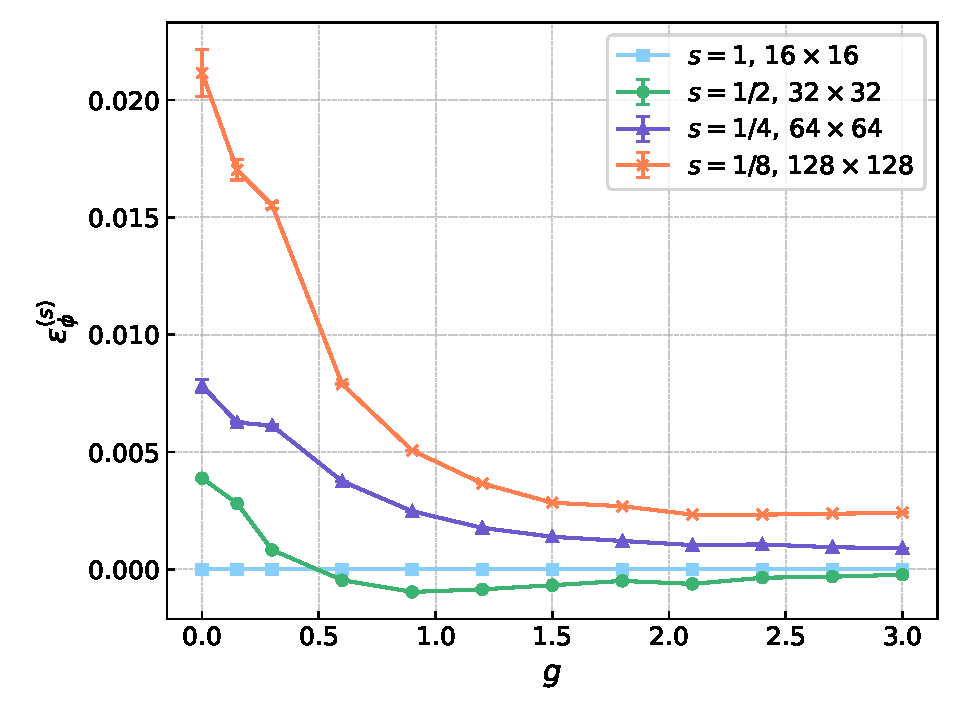
\includegraphics[width=\textwidth]{figures/cooling/yukawa_scan/deviation.pdf}
        \caption{Absolute magnetisation}
    \end{subfigure}
    \begin{subfigure}[b]{0.45\textwidth}
        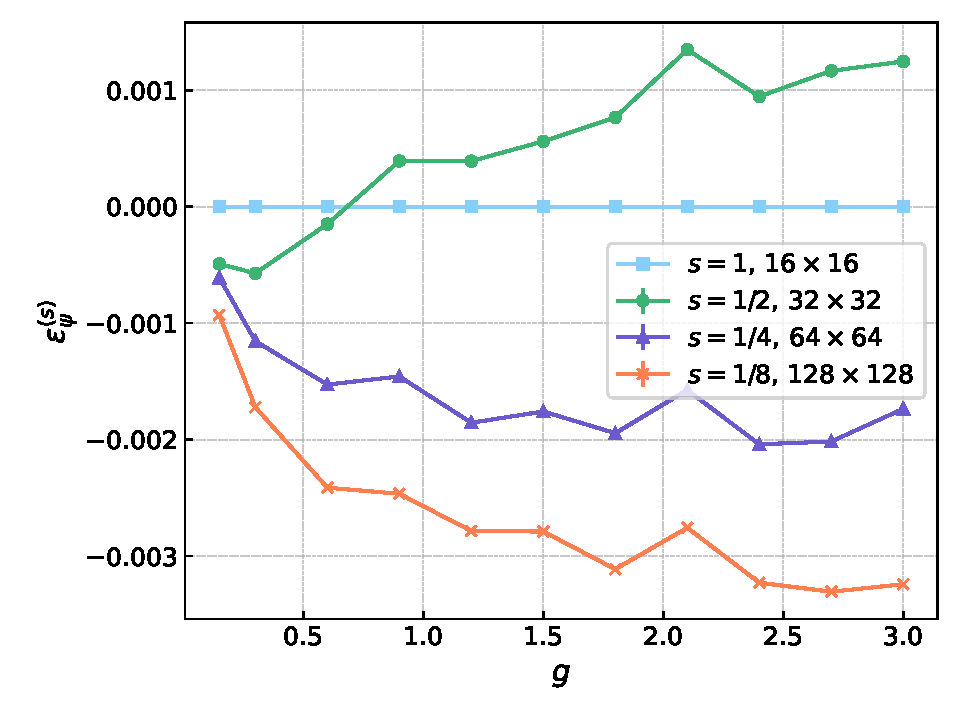
\includegraphics[width=\textwidth]{figures/cooling/yukawa_scan/deviation_cond.pdf}
        \caption{Chiral condensate}
    \end{subfigure}
    \caption[Relative error in the cooling procedure at tree level.]{Relative error of the absolute magnetisation and chiral condensate in the cooling procedure for various values of the noise fraction $s$.}
    \label{fig:cooling_deviation}
\end{figure}


\newpage





% !TeX root = ../main.tex

\chapter{Summary and outlook}
\label{chap:conclusions}
\section*{Summary}
In this thesis stochastic quantisation with coloured noise was introduced as a framework to control the momentum dependency of quantum fluctuations in a lattice field theory simulation. \\
Chapter \ref{chap:background} and Chapter \ref{chapt:methods} were devoted to the introduction of the relevant theoretical aspects and methodologies for this work. In particular, the formulation 
of stochastic quantisation in the presence of coloured noise resulted in a deep connection with the Wilsonian (functional) renormalisation group. \\
We then turned to the numerical analysis and experiments, applying the technique to a fermionic theory, a Yukawa model. In Chapter \ref{chapt:results_preliminary}, a preliminary analysis was carried out. The phase diagram of the theory showed that a proper phase transition in the model can happen only for vanishing Yukawa interaction due to the presence of Wilson 
fermions, which break chiral symmetry explicitly. Nevertheless, relevant features of the model such as the relation between magnetisation, chiral condensate, and fermionic mass, could be investigated. \\
After switching momentarily to the formulation with na\"ive fermions, removing the Wilson term, the behavior of the system in the presence of different noise degrees of freedom was studied and it was shown that for a particular combination of the bare parameters
a phase transition can happen while smoothly interpolating between the classical and quantum theories. \\
Finally, it was shown how the simulation can be cooled from ultraviolet degrees of freedom by encoding them in a redefinition of the bare couplings, performing block-spin transformations. It was shown that observables such as the magnetisation, chiral condensate, and magnetic susceptibility are not significantly altered in the coarse-graining procedure.
Other observables such as the scalar renormalised mass and fermionic pole mass, were shown to present some problems in the procedure. While the cause for the former has been elucidated and attributed to the choice of the regulating function for the noise term, more investigation is needed to understand the cause of the latter. 
\newpage 
\section*{Outlook}
The main result of this work is that the coarse-graining procedure via block-spin transformations was successfully applied to a fermionic theory. This adds another step towards a bigger goal, namely taking the continuum limit of a lattice low energy effective theory such as the Quark-Meson model. 
This would not only allow for a comparison between lattice results and functional methods, but would also remove the undesired effects of the Wilson term in the action. An interesting step forward starting from this work, would be to extend the investigation to systems at finite temperature and chemical potential. 
This could have particular benefits in lattice algorithms such as the Complex Langevin method, which aim at beating the sign problem, and often rely on cooling techniques for stabilisation. \\
An application of the algorithm to gauge theories would also be of great interest since the cooling procedure could then be applied to simulations of full QCD.  
In particular, we mention that an application in Yang-Mills theories could allow for a connection with the Wilson gradient flow of gauge links and allow for a precise control of the latter. Thus, this would be quite harder due to the fact that a momentum space cutoff breaks the gauge invariance of the theory.

%----------------------------------------------------------------------------------------
%	THESIS CONTENT - APPENDICES
%----------------------------------------------------------------------------------------

\appendix % Cue to tell LaTeX that the following "chapters" are Appendices

% Include the appendices of the thesis as separate files from the Appendices folder
% Uncomment the lines as you write the Appendices

% Appendix A

\chapter{Useful relations and definitions} % Main appendix title

\label{AppendixA} % For referencing this appendix elsewhere, use \ref{AppendixA}
In this appendix, useful relations and definitions are introduced.
Fermionic wo-points function
\begin{equation} 
\begin{aligned}
    \left\langle \psi_{s,f}(x) \, \bar\psi_{s',f'}(y) \right\rangle 
    &= \frac{1}{Z} \, \int \mathcal{D}\phi \, \mathcal{D}\psi \, \mathcal{D}\bar\psi \ \psi(x) \, \bar\psi(y) \, \exp \left( - S_\phi - \psi D \psi + \bar\eta \psi + \bar \psi \eta \right) \\
    &= \frac{1}{Z} \, \int \mathcal{D}\phi \, \mathcal{D}\psi \, \mathcal{D}\bar\psi \ \frac{\delta}{\delta \bar \eta(x)} \frac{\delta}{\delta \eta(y)} \, \exp \left( - S_\phi - \psi D \psi + \bar\eta \psi + \bar \psi \eta \right) \\
    &= \frac{1}{Z} \, \int \mathcal{D}\phi \ \text{det}\left[D(\phi)\right] \ \exp \left( - S_\phi \right) \ \frac{\delta}{\delta \bar \eta(x)} \frac{\delta}{\delta \eta(y)} \, \exp\left( \bar\eta D^{-1} \eta \right) \\
    &= \left\langle \left[D^{-1}(\phi)\right]_{s,s',f,f'}(x,y)\right\rangle
\end{aligned}
\label{eq:D_inv_condensate}
\end{equation}
The lattice version becomes
\begin{equation*}
     \left\langle \psi_m \, \bar\psi_n \right\rangle =     \left\langle \left[D^{-1}(\phi)\right]_{mn}\right\rangle
\end{equation*}
with $D$ beeing the Wilson Dirac operator. \\
From this, it follows straightforwardly
\begin{equation*}
    \left\langle  \bar\psi \psi \right\rangle = \underset{x,s,f}{\tr} D^{-1}
\end{equation*}
where $\left\langle  \bar\psi \psi \right\rangle = \underset{x,s,f}\sum  \left\langle \bar\psi_{s,f}(x) \, \psi_{s,f}(x) \right\rangle$. \\~\\
The correlator is defined as
\begin{align*}
    C(n_t,0) \equiv \frac{1}{N_x} \sum_{n_x} \left[\left\langle \psi(n_t, n_x) \, \bar\psi(0,0)\right\rangle + \left\langle \psi(N_t-n_t, n_x) \, \bar\psi(0,0) \right] \right\rangle
\end{align*}
Note that we sum up two waves because the source propagates both forward and backward in time due to the boundary conditions. \\
Since for $t \to \infty$ one has that $C(t,p) \propto e^{-E_0(p) t}$, we expect 
\begin{equation*}
    C(t,p) \approx \sinh \left(E_0 \left(\frac{N_t}{2} - t\right)\right)
\end{equation*}

Pole mass, renormalized mass, effective mass, bare mass, physical mass









Effective action
\begin{equation*}
    S_{\text{eff}} = S_\phi + \text{Tr} \log D(\phi)
\end{equation*}
Drift force
\begin{equation*}
    K_{\phi^j} = - \frac{\delta S}{\delta \phi^j} = - \frac{\delta S_\phi}{\delta \phi^j} - \text{Tr} \left[ D^{-1} \, \frac{\delta D}{\delta \phi^j} \right]
\end{equation*}


\chapter{Wilson fermions}
\label{AppendixB}

% !TeX root = ../main.tex
\chapter{Algorithms and technical details}
\label{chapt:AppendixC}

\section{Conjugate Gradient algorithm and the Dirac operator}
The full inversion of the Dirac operator is a very expensive computation, given that the Dirac operator has dimension $(2 \, N_t \, N_x \, N_f)^2$, even though it is very sparse and has only few non-zero entries. One can note that for the purpose of computing the fermionic contribution to the drift force and the extraction of the physical quark mass from the correlator (details in section x and section y), only the inverse operator applied to a vector is needed. Hence it is sufficient to compute 
\begin{equation}
    \psi = D^{-1} \left| \eta \right\rangle
    \label{Dirac_inversion_linear_system}
\end{equation}
Computing $\psi$ via equation \eqref{Dirac_inversion_linear_system} is equivalent to solve the linear system $D \psi = \eta$, which can be done efficiently by employing a method for sparse matrices such as Conjugate Gradient (CG) as explained in the following way.

We want to solve the equation
\begin{equation*} 
    D \, \psi = \eta
\end{equation*}
CG requires the matrix to be hermitian while D is only $\gamma^5$-hermitian (really? under which assumptions?). One can thus solve the linear system
\begin{equation*}
    \left(D D^{\dagger} \right) \xi = \eta
\end{equation*}
and then obtain $\psi$ by multiplying the solution $\xi$ by $D^{\dagger}$ since 
\begin{equation}
    D^{\dagger} \xi = D^{\dagger} \ \left(D D^{\dagger}\right)^{-1} \eta = D^{-1} \eta = \psi
\end{equation}
Analogously one can calculate
\begin{equation*}
    \chi = D^{\dagger} \eta
\end{equation*}
by solving
\begin{equation*}
    \left(D^{\dagger} D\right) \xi = \eta
\end{equation*}
and then applying $D$ to the result.

One can improve the solution via CG by solving a \emph{preconditioned} equation. Suppose that we want to solve the equation
\begin{equation*}
    M x = b
\end{equation*}
via CG. \\
Let us express the matrix $A$ as a block matrix
\begin{equation}
    M = \begin{pmatrix*}
        A & B \\ C & D
    \end{pmatrix*}
    \label{eq:block_matrix}
\end{equation}
We introduce the Schur complement of $M$
\begin{equation}
    M/D = A - B D^{-1} C
    \label{eq:schur_complement}
\end{equation}
This allows one to write $M$ (LDU decomposition, Gaussian elimination) as 

\begin{equation*}
M=\left[\begin{array}{ll}
A & B \\
C & D
\end{array}\right]=\left[\begin{array}{cc}
\mathbf{1}_p & -B D^{-1} \\
0 & \mathbf{1}_q
\end{array}\right]\left[\begin{array}{cc}
M / D & 0 \\
0 & D
\end{array}\right]\left[\begin{array}{cc}
\mathbf{1}_p & 0 \\
D^{-1} C & \mathbf{1}_q
\end{array}\right] = L A R
\end{equation*}

Which allows for an easy block inversion

\begin{equation*}
M^{-1} = \left[\begin{array}{cc}
I_p & 0 \\
-D^{-1} C & I_q
\end{array}\right]\left[\begin{array}{cc}
\left(A-B D^{-1} C\right)^{-1} & 0 \\
0 & D^{-1}
\end{array}\right]\left[\begin{array}{cc}
I_p & -B D^{-1} \\
0 & I_q
\end{array}\right]
= L^{-1} A^{-1} R^{-1}
\end{equation*}
The equation to solve now reads
\begin{equation*}
x = L^{-1} A^{-1} R^{-1} \ b \qquad \text{or} \qquad  y = A^{-1} c
\end{equation*}
with $y = L x$ and $c = R^{-1} b$. One can then solve the equation $y = A^{-1}c$ and get the solution $x$ by applying $L^{-1}$ to x. \\~\\
An example of preconditioning is the even-odd preconditioning. Let us write the dirac operator in the form of equation \eqref{eq:block_matrix} in the following way
\begin{equation*}
     M = \begin{pmatrix*}
        M_{ee} & M_{eo} \\ M_{oe} & M_{oo}
    \end{pmatrix*}
\end{equation*}
The Schur complement \eqref{eq:schur_complement} is 
\begin{equation*}
    \hat M \equiv M/M_{oo} = 
\end{equation*}

\section{Bilinear noise scheme}
\begin{equation*}
    \text{Tr} \left[ D^{-1} \, \frac{\delta D}{\delta \phi^j} \right] \approx \left\langle \eta \right|  D^{-1} \, \frac{\delta D}{\delta \phi^j} \left| \eta \right\rangle = 
    \left\langle \psi \right| \frac{\delta D}{\delta \phi^j} \left| \eta \right\rangle
    \qquad\qquad \left| \psi \right\rangle = D^{-1} \left| \eta \right\rangle = D^\dagger \, \underbrace{(D D^\dagger)^{-1} \left| \eta \right\rangle}_{\text{CG}}
\end{equation*}
\begin{equation}
    \tr {A} = \frac{1}{N} \ \lim_{N \to \infty} \sum_i^N \eta_i^T D_{ij} \eta_j
    \label{eq:bilinear_noise_scheme}
\end{equation}
where $\eta_i$ is a gaussian random field where each component is drawn from a normal distribution $\mathcal{N}(0,1)$. \\
More precisely each vector component $\eta_i^\alpha$ satisfies
\begin{equation*}
    \left\langle \eta_i^{\alpha} \right\rangle = 0 \qquad\qquad \left\langle \eta_i^{\alpha}\eta_j^{\beta} \right\rangle = \delta_{i,j} \, \delta^{\alpha \beta}
\end{equation*}
The series \eqref{eq:bilinear_noise_scheme} requires in principle an infinite number of vectors to evaluate the trace exactly. In practice we truncate it and choose $N=1$ \note{:D :D}. The average over Monte Carlo samples will eventually converge nevertheless to the right result. \\~\\



%----------------------------------------------------------------------------------------
%	BIBLIOGRAPHY
%----------------------------------------------------------------------------------------
\printbibliography[heading=bibintoc]

%----------------------------------------------------------------------------------------




%----------------------------------------------------------------------------------------
%	ABBREVIATIONS
%----------------------------------------------------------------------------------------

\begin{abbreviations}{ll} % Include a list of abbreviations (a table of two columns)

\textbf{RG} & \textbf{R}enormalisation \textbf{G}group\\
\textbf{fRG} & \textbf{F}unctional \textbf{R}enormalisation \textbf{G}group\\
\textbf{UV} & \textbf{U}ltra\textbf{v}iolet\\
\textbf{QFT} & \textbf{Q}uantum \textbf{F}ield \textbf{Theory}

\end{abbreviations}

%----------------------------------------------------------------------------------------
%	PHYSICAL CONSTANTS/OTHER DEFINITIONS
%----------------------------------------------------------------------------------------

\begin{constants}{lr@{${}={}$}l} % The list of physical constants is a three column table

% The \SI{}{} command is provided by the siunitx package, see its documentation for instructions on how to use it

Speed of Light & $c_{0}$ & \SI{2.99792458e8}{\meter\per\second} (exact)\\
%Constant Name & $Symbol$ & $Constant Value$ with units\\

\end{constants}

%----------------------------------------------------------------------------------------
%	SYMBOLS
%----------------------------------------------------------------------------------------

\begin{symbols}{lll} % Include a list of Symbols (a three column table)

%$a$ & distance & \si{\meter} \\
%$P$ & power & \si{\watt} (\si{\joule\per\second}) \\
%Symbol & Name & Unit \\

\addlinespace % Gap to separate the Roman symbols from the Greek

%$\omega$ & angular frequency & \si{\radian} \\

\end{symbols}



\end{document}  
